\documentclass[11pt]{article}

\usepackage[margin=1in]{geometry}
\usepackage{amsmath,amssymb}
\usepackage{booktabs}
\usepackage{graphicx}
\usepackage{hyperref}

\title{Robust and Non-Robust Features in a Fully Controlled Synthetic
Classification Task: A Minimal Demonstration}

\author{}
\date{}

\begin{document}
\maketitle

\begin{abstract}
Ilyas et al.\ (2019) argue that adversarial vulnerability arises because
standard training exploits any feature correlated with the label, including
\emph{non-robust} features that are predictive but brittle under small
perturbations, alongside \emph{robust} features that are predictive and
stable. We construct a minimal, fully controlled synthetic classification
task in which this distinction is explicit by design: one input dimension
determines the label deterministically (up to injected label noise) and five
additional dimensions are only probabilistically correlated with it. We show
that a standard multilayer perceptron trained on all six dimensions relies
measurably on the non-robust dimensions, that an attacker restricted to
perturbing only those dimensions is disproportionately effective, and that
removing the non-robust dimensions from the model's input entirely yields a
large improvement in adversarial robustness at a modest cost in clean
accuracy. We also report two negative/methodological findings from the
process of building this experiment: (i) the effect does not appear at all
unless the "robust" feature is made imperfect -- weight regularization,
which we initially thought was also required, turns out not to be, a
correction we only found by later sweeping the two factors independently
(see below) -- and (ii) a naive interpretation of a large attack budget
relative to the feature's dynamic range can be mistaken for a robustness
failure when it is simply a consequence of the budget size. We further
compare two forms of sparsity regularization as an alternative to
architected removal, and extend the setup to an image domain (a
convolutional network distinguishing circles from squares against a
partially-predictive gray background), which reproduces the core
phenomenon but also exposes a genuine disanalogy: when a robust feature is
spatially distributed across pixels rather than isolated in its own input
channel, restricting an attack to "that feature's region" is not the same
as restricting it to "that feature's channel," since the region's pixels
are the ground truth rather than a measurement of it. All quantitative
results are averaged over 10 random seeds and reported with standard
deviation; doing so surfaced a further finding of independent interest,
that the activation-sparsity failure mode of Section~\ref{sec:actsparsity}
is a seed-dependent knife-edge collapse rather than a fixed threshold, which
a single-seed evaluation would not have revealed. Because the generative
model is fully known, we also derive the exact Bayes-optimal classifier
and find the trained network relies on the jointly-informative but
individually-weak dimensions \emph{less} than is statistically optimal,
not more. An appendix subjects the main text's remaining choices to
broader checks: a multi-step PGD attack, a phase diagram over generative
and regularization parameters, a comparison against
$L_2$/group-Lasso/elastic-net/pruning alternatives, and an image
architecture with genuine per-cue channel separation rather than post-hoc
spatial masking. Code for all experiments is provided.
\end{abstract}

\section{Introduction}

Adversarial examples --- small, often imperceptible perturbations that
change a classifier's prediction --- are typically explained as artifacts of
model brittleness. Ilyas et al.\ \cite{ilyas2019} offer a different
account: standard supervised training has no preference for features that
are \emph{robust} (predictive and stable under small perturbation) over
features that are merely \emph{non-robust} (predictive but brittle). Both
reduce training loss, so both get used, and the non-robust ones are exactly
what an adversary exploits.

This account is usually demonstrated on real image data, where "robust" and
"non-robust" features cannot be enumerated or controlled directly. Our goal
here is much narrower: to construct the smallest possible synthetic task in
which the robust/non-robust distinction is a design choice rather than an
inference, so that the mechanism can be observed directly rather than
argued for indirectly.

This experiment was motivated by a broader question we do not attempt to
answer here: whether a model's measured \emph{equivariance} to known
physical transformations (rotation, scale, viewpoint) predicts whether an
adversarial perturbation crafted at one observation transfers naturally to
a transformed observation of the same object. The mechanistic link runs
through gradients: if a representation $z(x)$ is equivariant under a
transform $T$ (i.e.\ $z(T(x)) \approx A_T z(x)$ for some consistent operator
$A_T$), then by the chain rule the gradient $\nabla_x f(x)$ --- and hence an
attack built from it --- should transform predictably under $T$ as well.
Ilyas et al.'s robust/non-robust framing offers a plausible reason such an
operator $A_T$ might or might not exist: non-robust features are, by
construction, exactly the kind of brittle, high-frequency correlations
unlikely to transform predictably under a physical transformation, while
robust features are better candidates for being tied to real geometric
structure. Before pursuing that connection on real models and real
transformations, we wanted to see the more basic robust/non-robust
mechanism operating cleanly in a setting simple enough to fully control and
inspect. That is the contribution of this note.

\section{Related Work}

Szegedy et al.\ \cite{szegedy2014} first described adversarial examples for
deep networks. Goodfellow et al.\ \cite{goodfellow2015} introduced the Fast
Gradient Sign Method (FGSM), the single-step attack used throughout this
work; Madry et al.\ \cite{madry2018} generalized it to the iterative
Projected Gradient Descent (PGD) attack. Ilyas et al.\ \cite{ilyas2019}
proposed the robust/non-robust feature decomposition this paper takes as
its starting hypothesis, demonstrating it on ImageNet-scale data by
constructing datasets from purely non-robust features that nonetheless
generalize. Tsipras et al.\ \cite{tsipras2018} argue, separately, that
robustness and standard accuracy may be fundamentally at odds, a claim our
Model A/Model B accuracy gap reproduces in miniature. Athalye et al.\
\cite{athalye2018} showed that many defenses relying on input
transformation or randomization are broken once the attacker is allowed to
adapt (e.g.\ via Expectation over Transformation), which is why we do not
attempt to propose a defense in this note and restrict ourselves to
measurement.

\section{Synthetic Task}
\label{sec:task}

A terminological note before the construction: we use "robust" and
"non-robust" to name the two kinds of dimension, following
\cite{ilyas2019}, but the dimensions themselves are distinguished by a
purely \emph{statistical} property --- how reliably a dimension's value
determines $y$ under the generative model, i.e.\ $x_0$'s near-determinism
vs.\ $x_1,\ldots,x_5$'s weak correlation with $y$ (Table~\ref{tab:sanity})
--- not by any property of adversarial perturbation. "Non-robust" here
means "statistically weak, one dimension at a time," and the paper's
finding is that this statistical property is what predicts adversarial
vulnerability (Section~\ref{sec:main-result}), not that the label already
presupposes it. We keep Ilyas et al.'s terminology because our result is
a direct test of their claim under it, but Section~\ref{sec:bayes}'s
comparison to the Bayes-optimal classifier is exactly the check on whether
that statistical labeling is actually doing the explanatory work we
attribute to it, or merely restating the vulnerability gap in different
words.

Each example is a vector $x \in [0,1]^6$ with a binary label $y \in \{0,1\}$
drawn uniformly at random. The first dimension, $x_0$ (the \emph{signal}
dimension), is generated as
\[
x_0 = \mathrm{clip}(y + \varepsilon_0,\ 0, 1), \qquad \varepsilon_0 \sim
\mathcal N(0, \sigma_0^2),
\]
so that $x_0$ determines $y$ with high but not perfect reliability. The
remaining five dimensions $x_1,\dots,x_5$ (the \emph{noise} dimensions) are
each generated as
\[
x_i = \mathrm{clip}\big(0.5 + \alpha (y - 0.5) + \varepsilon_i,\ 0,
1\big), \qquad \varepsilon_i \sim \mathcal N(0, \sigma^2),
\]
so that each is only weakly, probabilistically correlated with $y$: its
mean shifts by $\alpha$ depending on the label, but the shift is small
relative to the noise. We use $\sigma_0 = 0.3$, $\alpha = 0.4$, $\sigma =
0.25$ throughout. A simple single-threshold classifier applied to $x_0$
alone achieves $95.2\%$ accuracy; applied to any single noise dimension
alone it achieves $78$--$79\%$ (Table~\ref{tab:sanity}). Neither is
deterministic, and $x_0$ is clearly the more reliable of the six. This is
also each dimension's exact Bayes-optimal single-dimension accuracy: for a
clipped-Gaussian pair with equal variance and means symmetric about $0.5$,
the midpoint threshold is Bayes-optimal, giving the closed form
$\Phi(\Delta\mu/2\sigma)$ ($\Phi$ the standard normal CDF, $\Delta\mu$ the
between-class mean gap) --- $\Phi(1/0.6)=0.9522$ for $x_0$ and
$\Phi(0.4/0.5)=0.7881$ for each noise dimension, both confirmed by direct
grid search on 2M samples (Section~\ref{sec:bayes}).

\begin{table}[h]
\centering
\caption{Best single-threshold accuracy achievable from each input
dimension alone, equal to that dimension's exact Bayes-optimal accuracy
(Section~\ref{sec:bayes}). None is deterministic; $x_0$ is the most
reliable. These follow directly from the fixed generative parameters
$\sigma_0, \alpha, \sigma$ (Section~\ref{sec:task}) rather than from a
trained model, so unlike every other table in this paper they carry no
seed variance (Section~\ref{sec:seeds}).}
\label{tab:sanity}
\begin{tabular}{lc}
\toprule
Dimension & Single-dimension accuracy \\
\midrule
$x_0$ (signal) & 0.952 \\
$x_1$ (noise) & 0.788 \\
$x_2$ (noise) & 0.788 \\
$x_3$ (noise) & 0.788 \\
$x_4$ (noise) & 0.788 \\
$x_5$ (noise) & 0.788 \\
\bottomrule
\end{tabular}
\end{table}

\section{Models}

All models are a single-hidden-layer MLP: a linear layer to 8 hidden
units, ReLU, and a linear output layer to 2 classes, trained with Adam
(learning rate $0.02$, 500 steps, weight decay $10^{-2}$) and
cross-entropy loss on 4{,}000 training examples, evaluated on 1{,}000 held-out
test examples.

\begin{itemize}
\item \textbf{Model A}: 6 real inputs. Trained on the full generative
process of Section~\ref{sec:task}.
\item \textbf{Model B}: 1 input. The five noise dimensions are removed
from the architecture entirely --- there is no input slot for them, and
therefore no attack surface associated with them, even in principle.
\item \textbf{Model C}: 6 input slots, but the five noise dimensions are
fixed at $0$ during both training and evaluation. Unlike Model B, the
architecture still has weights connecting these dimensions to the hidden
layer; those weights never receive gradient during training (since the
corresponding inputs are always $0$) and remain at their random
initialization. Model C tests whether this residual, untrained attack
surface is actually exploitable, as distinct from Model B's genuine
removal of it.
\end{itemize}

Figure~\ref{fig:arch} shows the three architectures schematically, with
input nodes colored by role: green for the robust signal dimension, orange
for the trained non-robust noise dimensions, and gray for dimensions that
are architecturally present but never receive training signal (Model C
only).

\begin{figure}[h]
\centering
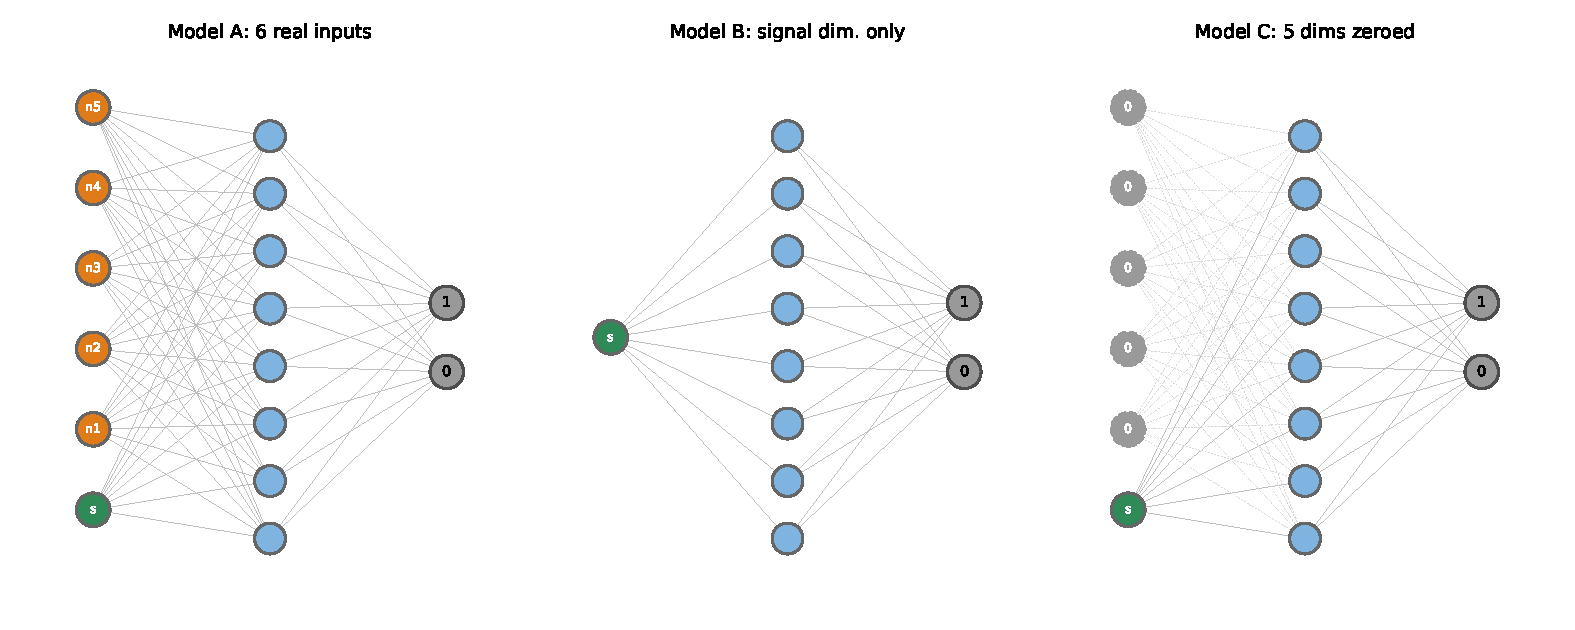
\includegraphics[width=0.95\textwidth]{fig_architectures.pdf}
\caption{The three architectures. Green: robust signal dimension. Orange:
trained non-robust noise dimensions (Model A only). Gray dashed (Model C):
input slots fixed at $0$, with connections that never receive a training
gradient. Model B has no slots for the noise dimensions at all. All three
share the same 8-unit ReLU hidden layer and 2-way softmax output.}
\label{fig:arch}
\end{figure}

\section{Attack Methodology}

We use single-step FGSM: given a correctly-classified point $x$ with label
$y$,
\[
x_{\mathrm{adv}} = \mathrm{clip}\big(x + \epsilon \cdot \mathrm{sign}\big(
\nabla_x \, \mathrm{CE}(f(x), y)\big) \odot m,\ 0, 1\big),
\]
where $m \in \{0,1\}^6$ is an optional mask restricting the attack to a
subset of dimensions ($m = \mathbf{1}$ for an unrestricted attack). Attack
success rate is the fraction of originally-correctly-classified test points
whose prediction changes after the perturbation. We report $\epsilon \in
\{0.02, 0.05, 0.10, 0.15, 0.20, 0.30\}$; we deliberately exclude
$\epsilon = 0.5$ from the main results, for reasons discussed in
Section~\ref{sec:pitfall}.

\subsection{Seeds and reported uncertainty}
\label{sec:seeds}

Every quantitative result below (all model accuracies, weight norms,
activation statistics, and attack success rates in
Sections~\ref{sec:main-result}--\ref{sec:actsparsity} and
Section~\ref{sec:image}) is computed independently for $N=10$ random seeds,
each reseeding both data sampling and model initialization, and reported as
mean $\pm$ one sample standard deviation across seeds. Table~\ref{tab:sanity}
is the one exception: those numbers are the best-threshold accuracy implied
directly by the fixed generative parameters $\sigma_0,\alpha,\sigma$, not an
estimate from a trained model, so they carry no seed variance. Two of the
two-sample illustrative diagnostics in Sections~\ref{sec:pilot} and
\ref{sec:pitfall}, and Figures~\ref{fig:arch}, \ref{fig:example},
\ref{fig:decision1d}, \ref{fig:decision1dA}, and \ref{fig:imageattack}, show
a single representative seed rather than a statistic, since they illustrate
one concrete instance (a decision function, an attacked example, a
diagram) rather than claim a quantitative effect size; this is noted again
at each occurrence. Running this experiment across seeds surfaced a
seed-dependent instability in Section~\ref{sec:actsparsity} that a
single-seed evaluation would have missed entirely -- see that section for
details.

\section{Results}

\subsection{The effect requires an imperfect signal}
\label{sec:pilot}

In an initial version of this experiment, the signal dimension was made
essentially noiseless ($\sigma_0 = 0.02$, single-dimension accuracy
$1.000$) and no weight decay was used. Under this configuration, the
trained model achieved $100\%$ clean accuracy and \emph{every} attack we
tried --- unrestricted, signal-only, or noise-only --- had a $0\%$ success
rate at every $\epsilon$ up to $0.3$, and only $4.9\%$ even at
$\epsilon=0.5$. The explanation is that when the signal dimension can drive
cross-entropy loss to (numerically) zero on its own, an unregularized
optimizer has no incentive to assign any meaningful weight to the noise
dimensions, so they end up carrying negligible learned weight and are not
exploitable regardless of budget. We initially fixed this by changing two
things at once --- making the signal dimension imperfect ($\sigma_0 =
0.3$, single-dimension accuracy $0.952$, not $1.0$) and adding weight
decay ($10^{-2}$) --- and attributed the fix to both. The phase-diagram
sweep in Appendix~\ref{app:phase} isolates the two factors and shows that
attribution was wrong: an imperfect signal alone, at \emph{zero} weight
decay, already produces substantial noise-dimension reliance
($\sigma_0=0.3, \alpha=0.4$: non-robust-only attack success $0.131$ at
$\epsilon=0.2$, five seeds, actually \emph{higher} than at
$\text{weight decay}=10^{-2}$'s $0.089$); weight decay was never the
active ingredient, and at fixed $\sigma_0$ increasing it mildly
\emph{reduces} noise-dimension reliance rather than enabling it, the
opposite of our original explanation. We keep weight decay in the main
text's models because it is still part of the exact configuration all our
numbers were computed under, not because it turned out to be necessary.
Section~\ref{sec:bayes} shows the noise dimensions' disuse in \emph{this}
pilot ($\sigma_0=0.02$) is not because they are only weakly informative in
some absolute sense --- each individually carries a real, substantial
likelihood-ratio weight under the true generative model, and combined they
carry \emph{more} than the signal dimension does --- so it is better read
as an artifact of cross-entropy loss saturating once the signal dimension
alone drives accuracy near $100\%$, not evidence that the noise dimensions
are statistically negligible. All results below use this corrected
configuration.

\subsection{A large attack budget is not a robustness test}
\label{sec:pitfall}

With the corrected configuration, an early version of Model B (six input
slots, noise dimensions zeroed, attack restricted to the signal dimension)
showed an attack success rate of $73.5\%$ at $\epsilon = 0.5$, which at
first reads as a robustness failure. We verified directly that this is a
budget artifact rather than a genuine vulnerability: the model's decision
boundary along the signal dimension sits at $x_0 \approx 0.487$, and
because $x_0 \in [0,1]$, \emph{every} correctly-classified test point is
within $L_\infty$ distance $0.5$ of that boundary by construction --- an
attacker with budget $0.5$ can reach the decision boundary from any point
in the domain, independent of whether the feature being attacked is robust
or not. (The gap between this $100\%$ reachability and the observed
$73.5\%$ success is explained by a clipping asymmetry: roughly half of the
label-1 examples are clipped to exactly $x_0 = 1.0$, and a full $-0.5$ step
from there lands at $x_0 = 0.5$, just short of crossing back over the
$0.487$ boundary.) We conclude that $\epsilon = 0.5$ is not a meaningful
budget for this task --- it spans half the feature's entire dynamic range
--- and exclude it from the main comparison.

Figure~\ref{fig:decision1d} shows the underlying picture directly rather
than only in numbers: the two class-conditional distributions (histograms)
overlap substantially and pile up at the clipping boundaries $0$ and $1$,
the model's learned $P(\text{class}=1)$ curve is a smooth sigmoid crossing
$0.5$ near the reported boundary, and an arrow of length $0.5$ from $x=0$
reaches that boundary directly, independent of any property of the
feature other than the domain being $[0,1]$.

\begin{figure}[h]
\centering
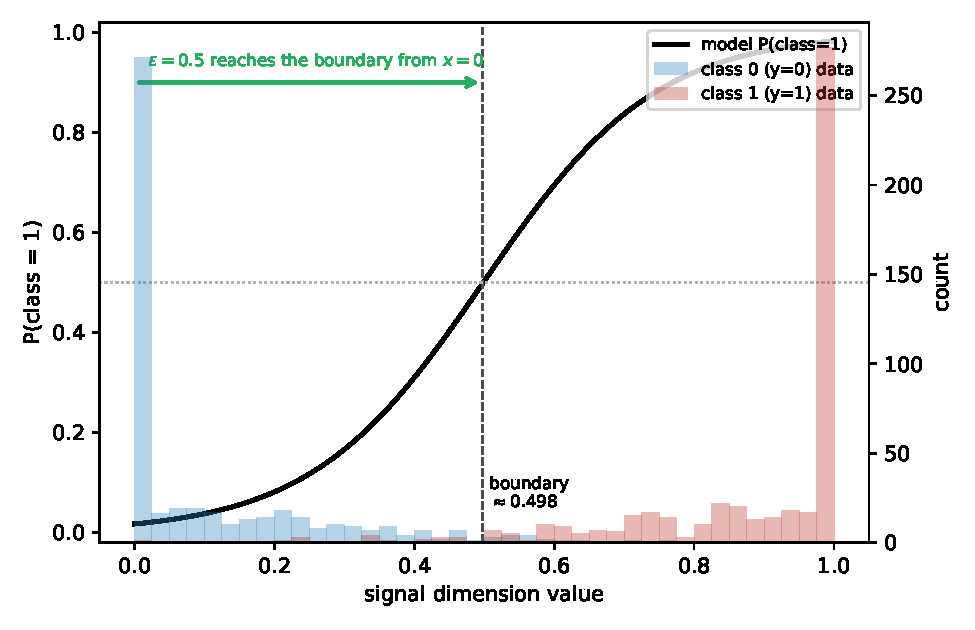
\includegraphics[width=0.72\textwidth]{fig_decision_1d_modelb.pdf}
\caption{Model B's decision function (black) over its single input
dimension, with the class-conditional data distributions (histograms,
right axis). Every point in $[0,1]$ is within $\epsilon=0.5$ of the
decision boundary by construction, regardless of feature reliability.}
\label{fig:decision1d}
\end{figure}

\subsection{Main result: locating and removing the non-robust attack surface}
\label{sec:main-result}

Table~\ref{tab:main} reports attack success rate as a function of $\epsilon$
for Models A, B, and C, with Model A additionally broken down by which
dimensions the attacker is allowed to perturb.

\begin{table}[h]
\centering
\caption{Attack success rate by model, restriction, and budget: mean
$\pm$ std over 10 seeds (Section~\ref{sec:seeds}). Clean test accuracy:
Model A $0.992\pm0.003$, Model B $0.954\pm0.007$, Model C $0.955\pm0.005$.}
\label{tab:main}
\begin{tabular}{lcccccc}
\toprule
$\epsilon$ & A: all dims & A: robust only & A: non-robust only & B: robust only & C: all dims & C: dead dims only \\
\midrule
0.02 & 0.005$\pm$0.002 & 0.002$\pm$0.001 & 0.003$\pm$0.002 & 0.006$\pm$0.003 & 0.006$\pm$0.002 & 0.000$\pm$0.000 \\
0.05 & 0.015$\pm$0.005 & 0.004$\pm$0.002 & 0.009$\pm$0.004 & 0.019$\pm$0.005 & 0.018$\pm$0.005 & 0.000$\pm$0.000 \\
0.10 & 0.051$\pm$0.009 & 0.009$\pm$0.004 & 0.025$\pm$0.007 & 0.044$\pm$0.008 & 0.042$\pm$0.005 & 0.000$\pm$0.000 \\
0.15 & 0.118$\pm$0.012 & 0.015$\pm$0.005 & 0.050$\pm$0.009 & 0.076$\pm$0.011 & 0.075$\pm$0.006 & 0.000$\pm$0.000 \\
0.20 & 0.241$\pm$0.014 & 0.025$\pm$0.006 & 0.086$\pm$0.012 & 0.117$\pm$0.014 & 0.113$\pm$0.010 & 0.000$\pm$0.000 \\
0.30 & 0.667$\pm$0.024 & 0.052$\pm$0.009 & 0.224$\pm$0.023 & 0.215$\pm$0.015 & 0.211$\pm$0.013 & 0.000$\pm$0.000 \\
\bottomrule
\end{tabular}
\end{table}

\begin{figure}[h]
\centering
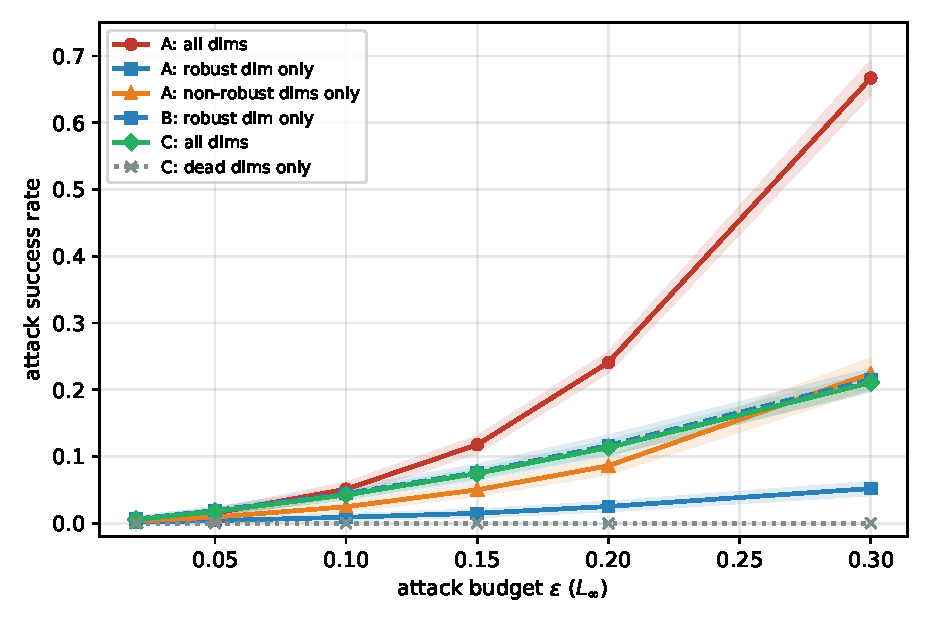
\includegraphics[width=0.72\textwidth]{fig_epsilon_curves.pdf}
\caption{Attack success rate vs.\ $L_\infty$ budget $\epsilon$, all six
series from Table~\ref{tab:main}; solid lines are the across-seed mean and
shaded bands are $\pm 1$ standard deviation over the same 10 seeds. The
non-robust-only curve for Model A (orange) rises well above its
robust-only curve (blue solid) at every budget; Model B (blue dashed)
stays close to Model A's robust-only curve; Model C's dead-dims curve
(gray) is flat at zero throughout, with zero variance across every seed.}
\label{fig:curves}
\end{figure}

Figure~\ref{fig:decision1dA} shows why the two channels behave so
differently, by slicing Model A's decision function along each input
dimension in turn (holding the other five at their test-set mean). The
signal panel is a steep, well-separated sigmoid tracking the two
histograms closely; every noise panel is a shallow, near-linear ramp
running through two heavily overlapping histograms. The weight-norm
asymmetry reported earlier is the same fact expressed as a single number
per dimension; this is what it looks like as a function.

\begin{figure}[h]
\centering
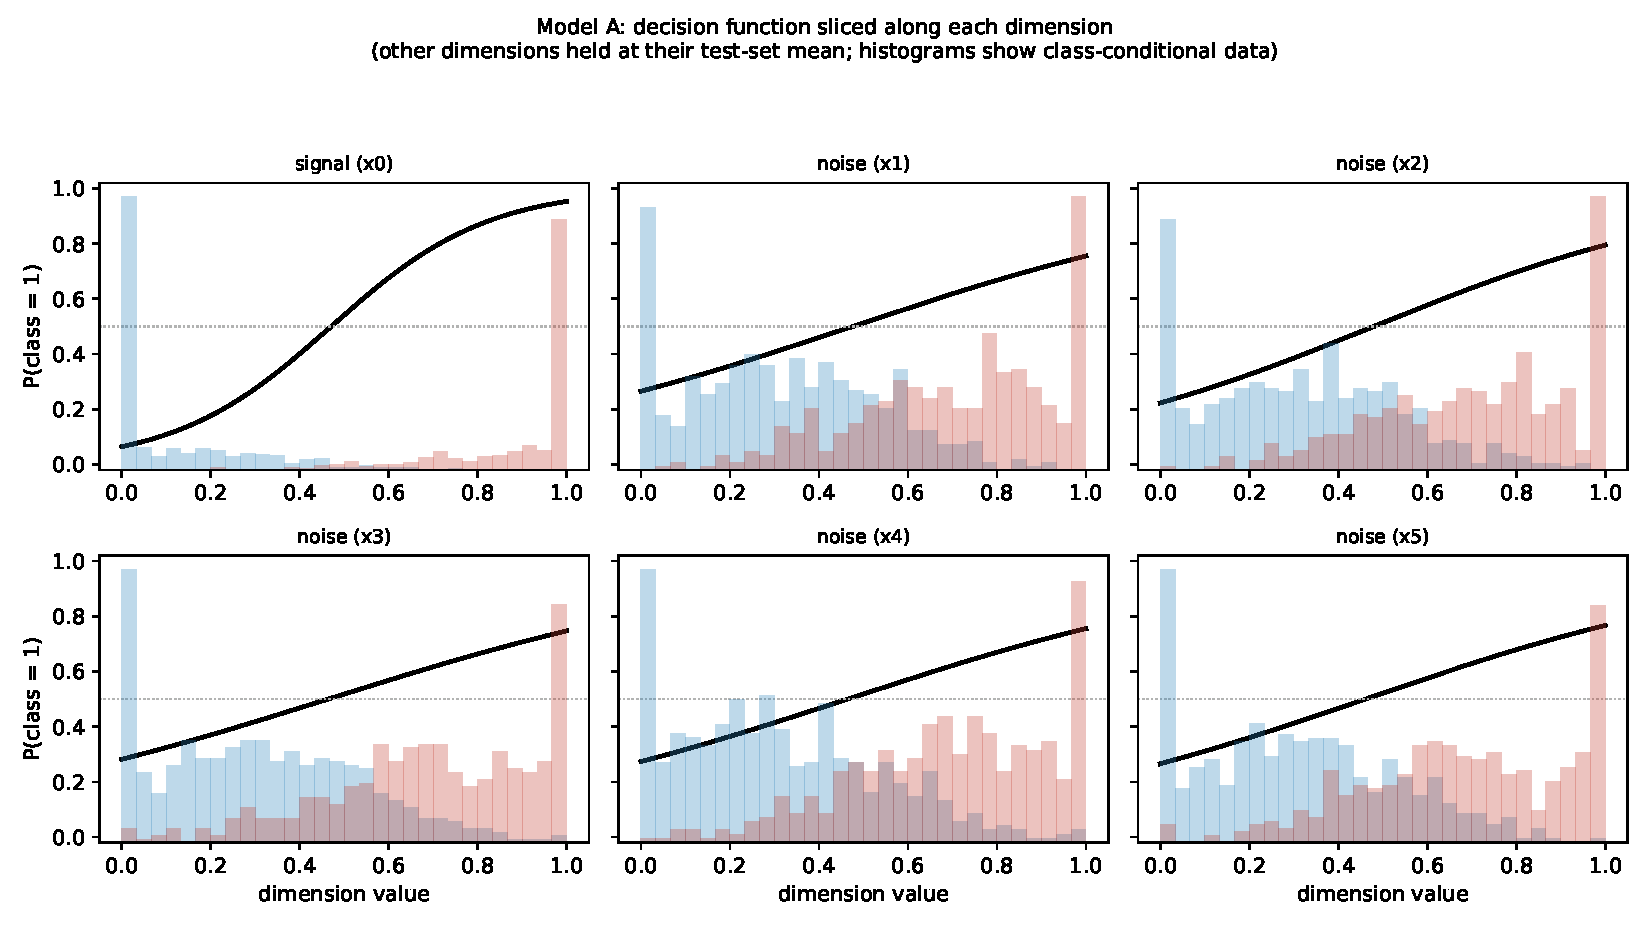
\includegraphics[width=\textwidth]{fig_decision_1d_modela_allDims.pdf}
\caption{Model A's decision function sliced along each of the six input
dimensions (other dimensions held at their test-set mean), with
class-conditional data histograms overlaid. The signal dimension alone
produces a sharp, well-separated curve.}
\label{fig:decision1dA}
\end{figure}

Three patterns are visible. First, for Model A, restricting the attacker to
the five non-robust dimensions is consistently 2--4$\times$ more effective
than restricting it to the single robust dimension, at every budget (e.g.\
$0.224\pm0.023$ vs.\ $0.052\pm0.009$ at $\epsilon = 0.3$) --- the model's
vulnerability is concentrated in the dimensions that were only ever
probabilistically correlated with the label, not the one that determined
it. Second, an unrestricted attacker does better than either restricted
subset alone ($0.667\pm0.024$ at $\epsilon = 0.3$), consistent with
combining both channels. Third, and this is the main result, Model B is
substantially harder to fool than Model A at every budget from
$\epsilon=0.05$ upward (e.g.\ $0.215\pm0.015$ vs.\ $0.667\pm0.024$ at
$\epsilon=0.3$), at the cost of $3.8$ points of clean accuracy
($99.2\%\pm0.3\to95.4\%\pm0.7$) --- removing the non-robust dimensions from
the model's input, rather than merely restricting an attacker's access to
them post hoc, yields a real and fairly large robustness improvement, and
this holds consistently across all 10 seeds (the standard deviations above
are all small relative to the effect size).

Figure~\ref{fig:example} makes this concrete with one actual test example
per model, at $\epsilon = 0.3$, rather than an aggregate rate. For Model A
under a noise-only attack, the signal dimension (leftmost bar pair) is
untouched by construction, while all five noise dimensions shift --- and
that shift alone is enough to flip the prediction despite the untouched
signal dimension still correctly indicating the true label. For Model B,
the only dimension it has is pushed by the full budget and crosses its
decision boundary.

\begin{figure}[h]
\centering
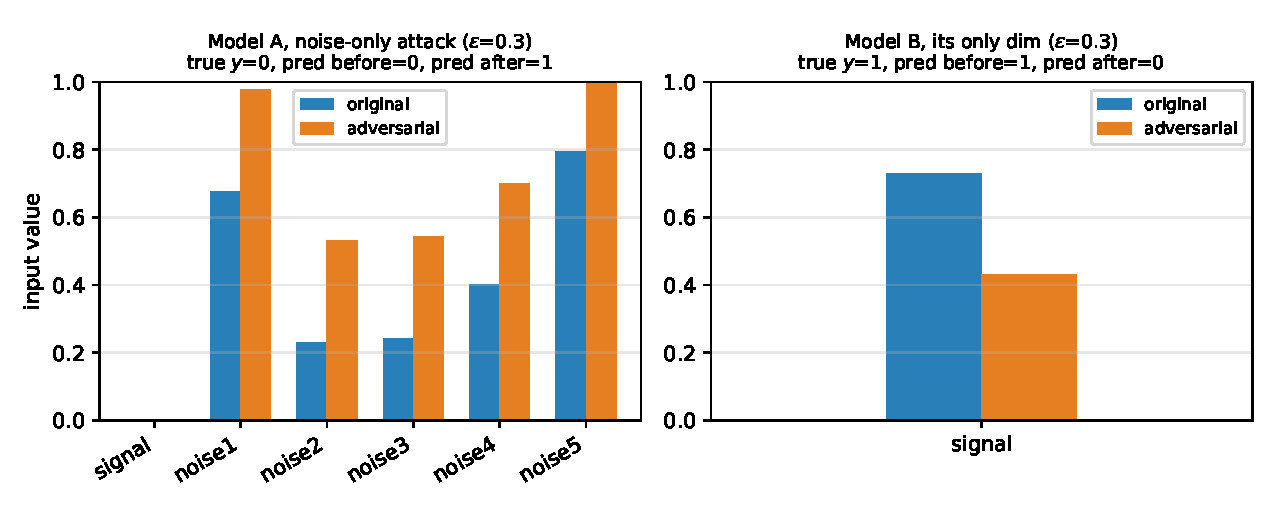
\includegraphics[width=0.95\textwidth]{fig_example_attack.pdf}
\caption{One concrete successful attack per model at $\epsilon=0.3$,
showing the actual input vector before and after perturbation. Left: Model
A, attack restricted to the five non-robust dimensions only --- the
signal dimension is unchanged, yet the combined shift in the noise
dimensions still flips the prediction. Right: Model B, whose only
dimension is perturbed directly.}
\label{fig:example}
\end{figure}

\subsection{Comparison to the Bayes-optimal classifier}
\label{sec:bayes}

Every number above describes a trained MLP; because the generative process
is fully known, we can also compute the exact Bayes-optimal classifier for
any subset of input dimensions and ask whether the MLP's reliance on the
non-robust dimensions reflects a real statistical incentive or an
optimization artifact. For dimensions generated as a clipped Gaussian
whose mean shifts with $y$ and whose variance does not, the log-likelihood
ratio is linear in $x$ in the interior of $[0,1]$ and takes the boundary
mass ratio at the two endpoints; summing this exactly across dimensions
(valid since they are conditionally independent given $y$ by construction)
gives the exact Bayes rule for any subset, which we evaluate here by Monte
Carlo (code in \texttt{bayes\_optimal\_analysis.py}).

\begin{table}[h]
\centering
\caption{Bayes-optimal accuracy for different input subsets ($N=200{,}000$
Monte Carlo samples; binomial standard error $\lesssim 0.001$ throughout,
since this is a fixed population quantity, not a trained-model estimate),
vs.\ the trained MLP (Model A, mean over 10 seeds).}
\label{tab:bayes}
\begin{tabular}{lc}
\toprule
Classifier & Accuracy \\
\midrule
Bayes-optimal, all 6 dims & 0.9926 \\
Bayes-optimal, $x_0$ only & 0.9522 \\
Bayes-optimal, 5 noise dims combined & 0.9630 \\
Bayes-optimal, 1 noise dim only & 0.7878 \\
\midrule
Trained MLP (Model A), all 6 dims & $0.992\pm0.003$ \\
\bottomrule
\end{tabular}
\end{table}

Two things stand out. First, Model A's clean accuracy ($0.992\pm0.003$) is
statistically indistinguishable from the Bayes optimum ($0.9926$) --- on
raw accuracy, the trained MLP is not leaving anything on the table.
Second, and this is the more surprising number, the five noise dimensions
\emph{combined optimally} reach $96.3\%$ accuracy on their own, comfortably
above any single noise dimension's $78.8\%$ and not far below the signal
dimension's $95.2\%$: five conditionally-independent partial measurements
of the same underlying label-correlation combine to be substantially more
informative than any one of them looked at alone. Converting each
channel's exact log-likelihood-ratio weight per unit input into a single
number (ignoring the boundary correction, which is small here) gives
$11.11$ for the signal dimension and $6.40$ per noise dimension, i.e.\
$32.0$ for the five combined --- so a Bayes-optimal classifier would place
\emph{more} total evidential weight on the noise channel than on the
signal channel ($2.88{:}1$), not less. The noise dimensions are not weak
because they carry little information; they are weak only one at a time.

This reframes the question the rest of this paper asks. Model A's
first-layer weight norm ratio favors the signal dimension by
$\approx 2.4{:}1$ (Section~\ref{sec:sparsity}), the opposite direction
from the Bayes-optimal ratio above --- but weight norms in a nonlinear
network are not the same object as a linear log-likelihood weight, so we
compare the two classifiers on a common, model-agnostic footing instead:
permutation importance, i.e.\ the accuracy drop from independently
shuffling a channel's values across the test set (breaking its
correlation with $y$) and re-applying the otherwise-unchanged decision
rule. We compute this for both the Bayes-optimal rule and Model A, on the
same 10 seeds' test sets, shuffling either $x_0$ alone or all five noise
dimensions jointly.

\begin{table}[h]
\centering
\caption{Permutation-importance accuracy drop, Bayes-optimal vs.\ trained
MLP (Model A): mean $\pm$ std over 10 seeds.}
\label{tab:permimportance}
\begin{tabular}{lccc}
\toprule
Classifier & Signal permuted & Noise permuted & Noise:signal ratio \\
\midrule
Bayes-optimal & $0.196\pm0.008$ & $0.154\pm0.006$ & $0.79$ \\
Trained MLP (Model A) & $0.275\pm0.006$ & $0.100\pm0.009$ & $0.36$ \\
\bottomrule
\end{tabular}
\end{table}

The answer to the question this section opened with is: no, if anything
the opposite. The Bayes-optimal classifier's own permutation-importance
ratio is $0.79$ --- shuffling the noise channel costs it nearly as much
accuracy as shuffling the signal dimension, consistent with the
near-parity of evidential weight computed above. Model A's ratio is
$0.36$: it depends on the noise channel distinctly \emph{less}, relative
to its dependence on the signal dimension, than a statistically optimal
classifier would. This does not contradict the rest of the paper --- Model
A's reliance on the noise channel is still real, still large enough in
absolute terms to be the dominant attack surface (Table~\ref{tab:main}),
and still concentrated disproportionately on those five dimensions per
unit of input perturbation. But in relative terms, gradient descent under
cross-entropy loss and $L_2$ weight decay under-uses the jointly
informative noise channel compared to what the known generative model
would justify, rather than over-fitting to it. We would not assume this
direction of miscalibration generalizes beyond this specific loss,
optimizer, and regularization strength; it is itself an empirical finding
of this comparison, not a property we derived independently of it.

\subsection{Naive zeroing versus true dimensionality reduction}

Model C tests whether that improvement requires physically removing the
non-robust dimensions from the architecture, or whether simply training
with them fixed at zero is enough. A priori this was unclear: the weights
connecting those dimensions to the hidden layer are never trained (they
receive no gradient when their input is always $0$) and remain at random
initialization, which could in principle be exploited by perturbing those
nominally "zeroed" inputs away from $0$ at attack time. Empirically, this
did not happen: \texttt{C: dead dims only} is exactly $0.000\pm0.000$ at
every $\epsilon$ we tested, in every one of the 10 seeds, and \texttt{C:
all dims} tracks \texttt{B: robust only} closely ($0.211\pm0.013$ vs.\
$0.215\pm0.015$ at $\epsilon=0.3$) rather than anything close to Model A.
In this task, at these budgets, naive zeroing during training was
empirically indistinguishable from true architectural removal, and this
held with zero variance across seeds. We flagged this as possibly
initialization-dependent rather than a general property, and rather than
leave that as a caveat we tested it directly (code in
\texttt{model\_c\_robustness.py}).

Because the dead dimensions are always exactly $0$ at input, their
first-layer weight columns receive an exactly-zero gradient regardless of
their value (the weight gradient is an outer product with the input),
so whatever we set those columns to at initialization is exactly what
they still are after training. This lets us deliberately construct
dead-feature weights rather than merely accepting whatever random
initialization produced. We tried three constructions, still on all 10
seeds: (i) scaling the default random initialization of the dead columns
by $3\times$, $10\times$, and $100\times$; (ii) replacing them with an
\emph{adversarial} but realistic choice --- the actual first-layer weights
a same-seed, fully-trained Model A learned for those same five dimensions,
i.e.\ weights we know are informative when the corresponding input
actually varies; and (iii) repeating both on a linear model (no hidden
layer) with the same zeroing setup, where the mechanism is fully
transparent analytically.

The random-scaling sweep (Table~\ref{tab:modelc}) shows this is indeed
initialization-scale-dependent, just not within the range ordinary random
initialization occupies: $3\times$ and $10\times$ the default scale leave
attack success at essentially $0$ ($\le 0.001$), but $100\times$ makes the
dead dimensions dramatically exploitable ($0.81\pm0.21$ at
$\epsilon=0.3$, rising to $0.22\pm0.12$ already at $\epsilon=0.02$). The
adversarial construction (ii), by contrast, remained exactly
$0.000\pm0.000$ at every $\epsilon$ we tested, across all 10 seeds ---
despite using weights we know encode real predictive information, just
not large ones: a same-seed Model A's learned noise-dimension weight norm
($\approx 0.6$) turns out to be about the same order of magnitude as the
default random initialization's norm ($0.648\pm0.056$ over the same 10
seeds), not $100\times$ larger, so transplanting it does not cross the
threshold the scaling sweep identifies.

\begin{table}[h]
\centering
\caption{Model C dead-dims-only attack success at $\epsilon=0.3$ under
different constructions of the (always architecturally-frozen) dead-input
weight columns: mean $\pm$ std over 10 seeds. Clean accuracy is unaffected
by any of these (it depends only on the trained signal-dimension weight),
staying at $0.955\pm0.005$ throughout.}
\label{tab:modelc}
\begin{tabular}{lc}
\toprule
Dead-weight construction & Attack success, $\epsilon=0.3$ \\
\midrule
default random init & $0.000\pm0.000$ \\
$3\times$ default scale & $0.000\pm0.000$ \\
$10\times$ default scale & $0.001\pm0.001$ \\
$100\times$ default scale & $0.811\pm0.215$ \\
adversarial (matched Model A weights) & $0.000\pm0.000$ \\
\bottomrule
\end{tabular}
\end{table}

The linear-model version (iii) makes the mechanism exact rather than
merely plausible. With no hidden layer, FGSM's worst-case shift in a
logit from perturbing the dead dimensions is exactly $\epsilon \cdot
\lVert W_{\text{dead}} \rVert_1$ (the L1 norm is exact here because
sign-based perturbation saturates each term of that norm simultaneously);
a point misclassifies once this exceeds its pre-attack margin between the
two class logits. This predicts a magnitude threshold with no reference to
activation states at all, and the data confirm it: attack success stays
at $0.000$ at $10\times$ scale, is still negligible at $30\times$
($0.003\pm0.003$), and becomes large by $100\times$ ($0.692\pm0.226$),
climbing further at $300\times$ and $1000\times$ ($0.85$ and $0.90$).
The MLP's qualitatively identical transition (Table~\ref{tab:modelc}) is
therefore not a distinct, activation-dependent phenomenon --- it is the
same weight-magnitude threshold, with the ReLU hidden layer adding only a
constant-factor correction, not a qualitatively different mechanism.

The overall picture is more precise than the original single-seed claim.
Model C's dead dimensions are not safe because they are architecturally
frozen, and not safe merely because a particular random seed happened to
leave them unexploited; they are safe because their weight
\emph{magnitude} sits well below the threshold a bounded attack budget
needs to move a typical point's logit margin, and this holds equally for
a genuinely informative weight vector transplanted from a real trained
model, as long as its magnitude is unremarkable. Freezing an input at
zero does not, on its own, guarantee safety at any weight scale; it
guarantees safety only in the (here, large) regime of weight scales where
the resulting worst-case logit shift stays below the decision margin,
a regime that both random initialization and realistic learned solutions
happened to fall well inside for this task.

\subsection{Discovered sparsity versus architected sparsity}
\label{sec:sparsity}

Sections~\ref{sec:pilot}--\ref{sec:main-result} removed the non-robust
dimensions by construction (Model B) or by fixing their value during
training (Model C). A natural question is whether a model can find a
similar solution on its own, without us deciding in advance which
dimension is reliable, simply by imposing a sparsity-inducing penalty and
letting the optimizer discover which features are worth keeping. We add an
$L_1$ penalty on the first layer's weights to the training objective,
\[
\mathcal L = \mathrm{CE}(f(x), y) + \lambda_{L_1} \lVert W^{(1)} \rVert_1,
\]
in place of the $L_2$ weight decay used for Model A, and call the result
Model A-sparse. This is the classical Lasso feature-selection mechanism
\cite{tibshirani1996} applied to a first layer whose columns correspond to
input dimensions, so we can inspect exactly which dimensions it selects.

Our first attempt used $\lambda_{L_1} = 0.02$ and appeared to show no
effect: Model A-sparse's ratio of signal-dimension to mean-noise-dimension
weight norm ($\approx 2.6$) was almost identical to Model A's under plain
$L_2$ decay ($\approx 2.4$), and its overall attack success rate was not
lower. This turned out to be a coincidence of scale, not a negative
result about $L_1$ regularization: sweeping $\lambda_{L_1}$ against a
true no-regularization baseline (Figure~\ref{fig:l1sweep}, mean over 10
seeds) shows the signal:noise weight ratio climbing steadily and
substantially --- from $\approx 1.4$ with no regularization at all, past
$\approx 2.6$ at $\lambda_{L_1}=0.02$ (which is why that value looked
unremarkable), up to $\approx 20$ at $\lambda_{L_1}=0.4$. $L_1$
regularization does perform real feature selection here;
$\lambda_{L_1}=0.02$ was simply too weak to reveal it, and comparing it
against the $L_2$ model rather than the unregularized baseline obscured
the trend on the first attempt. At the largest value tested,
$\lambda_{L_1}=0.8$, the sweep also shows the one place this mechanism
becomes seed-dependent rather than uniform: in 2 of the 10 seeds the
penalty over-shrinks the signal dimension itself, not just the noise
dimensions (signal weight norm collapsing to $\approx 0.01$--$0.02$,
against $\approx 0.23$--$0.29$ for the other 8 seeds), which is why the
signal-norm error bar widens sharply at that point in
Figure~\ref{fig:l1sweep} and the mean signal:noise ratio there
($\approx 18$) is, misleadingly, lower than at $\lambda_{L_1}=0.4$ despite
the noise norm continuing to shrink. We do not use $\lambda_{L_1}=0.8$
below for this reason.

\begin{figure}[h]
\centering
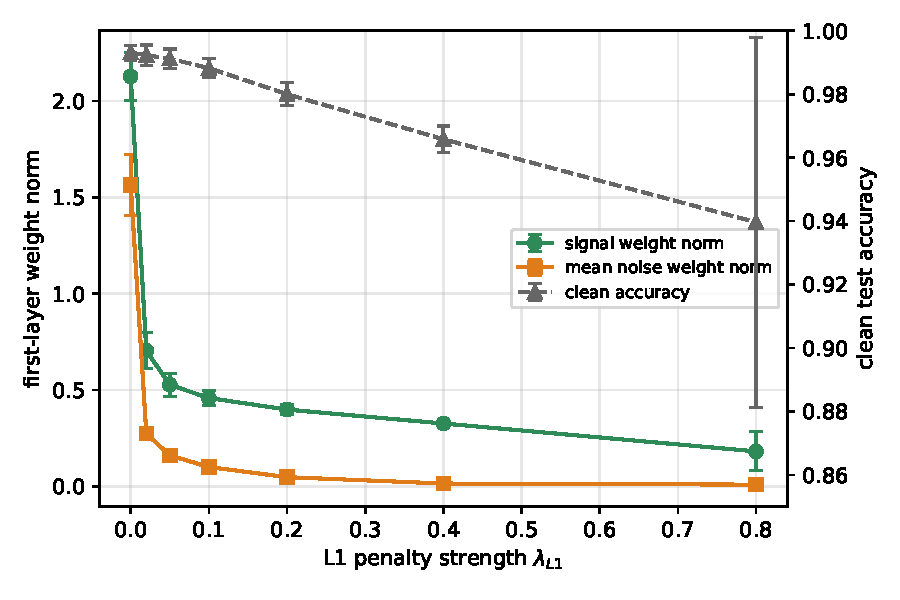
\includegraphics[width=0.62\textwidth]{fig_l1_sweep.pdf}
\caption{First-layer weight norm on the signal dimension vs.\ the mean over
the five noise dimensions, as $L_1$ penalty strength increases (left axis),
alongside clean test accuracy (right axis, dashed); error bars are
$\pm 1$ std over 10 seeds. The gap between the two solid curves widens by
more than an order of magnitude as $\lambda_{L_1}$ grows, while accuracy
degrades only mildly, until $\lambda_{L_1}=0.8$ where a minority of seeds
over-shrink the signal weight itself (visible as the widened error bar).}
\label{fig:l1sweep}
\end{figure}

We select $\lambda_{L_1} = 0.4$, which drives Model A-sparse's clean
accuracy to $96.6\%\pm0.6$ --- reasonably close to, though not exactly
matching, Model B's $95.4\%\pm0.7$, so the comparison below is at broadly
similar rather than precisely matched accuracy. Table~\ref{tab:sparse} and
Figure~\ref{fig:sparsecurves} compare the resulting attack surface against
Model A and Model B.

\begin{table}[h]
\centering
\caption{Attack success rate, Model A vs.\ Model A-sparse
($\lambda_{L_1}=0.4$), vs.\ Model B: mean $\pm$ std over 10 seeds. Clean
accuracy: A $0.992\pm0.003$, A-sparse $0.966\pm0.006$, B $0.954\pm0.007$.}
\label{tab:sparse}
\begin{tabular}{lccccc}
\toprule
$\epsilon$ & A: all dims & As: all dims & As: robust only & As: non-robust only & B: robust only \\
\midrule
0.02 & 0.005$\pm$0.002 & 0.007$\pm$0.003 & 0.006$\pm$0.003 & 0.001$\pm$0.001 & 0.006$\pm$0.003 \\
0.05 & 0.015$\pm$0.005 & 0.019$\pm$0.005 & 0.015$\pm$0.004 & 0.003$\pm$0.001 & 0.019$\pm$0.005 \\
0.10 & 0.051$\pm$0.009 & 0.046$\pm$0.007 & 0.036$\pm$0.007 & 0.006$\pm$0.002 & 0.044$\pm$0.008 \\
0.15 & 0.118$\pm$0.012 & 0.082$\pm$0.005 & 0.065$\pm$0.006 & 0.009$\pm$0.003 & 0.076$\pm$0.011 \\
0.20 & 0.241$\pm$0.014 & 0.128$\pm$0.011 & 0.095$\pm$0.009 & 0.013$\pm$0.005 & 0.117$\pm$0.014 \\
0.30 & 0.667$\pm$0.024 & 0.242$\pm$0.020 & 0.182$\pm$0.015 & 0.018$\pm$0.008 & 0.215$\pm$0.015 \\
\bottomrule
\end{tabular}
\end{table}

\begin{figure}[h]
\centering
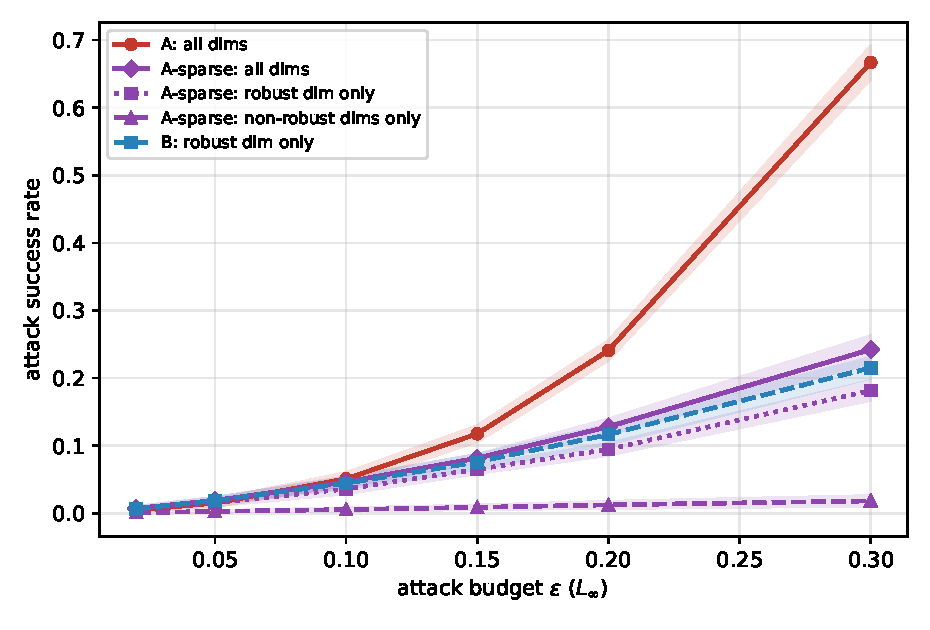
\includegraphics[width=0.72\textwidth]{fig_sparse_curves.pdf}
\caption{Attack success rate vs.\ budget for Model A, Model A-sparse
(overall and split by channel), and Model B; shaded bands are $\pm 1$ std
over 10 seeds. Model A-sparse's overall curve (purple, all dims) sits close
to Model B's (blue dashed) at every budget, despite Model A-sparse still
architecturally having all six input slots.}
\label{fig:sparsecurves}
\end{figure}

Two things are worth separating out. First, the headline effect: at
$\epsilon=0.3$, \texttt{As: all dims} ($0.242\pm0.020$) is close to
\texttt{B: robust only} ($0.215\pm0.015$) and far below \texttt{A: all
dims} ($0.667\pm0.024$) --- a model that discovers sparsity on its own
recovers most of the robustness benefit that we obtained in Model B by
deciding, ourselves, which dimension to keep. This did not require
knowing in advance which of the six dimensions was reliable.

Second, the mechanism is not simply "the non-robust channel became as safe
as it was for Model B." Restricting the attacker to the non-robust
dimensions alone (\texttt{As: non-robust only}, $0.018\pm0.008$ at
$\epsilon=0.3$) is in fact substantially safer than that channel was for
Model A ($0.224\pm0.023$) --- roughly a $12\times$ reduction --- but
restricting the attacker to the signal dimension alone (\texttt{As:
robust only}, $0.182\pm0.015$) is \emph{less} safe than the same
restriction was for Model A ($0.052\pm0.009$). This mirrors the asymmetry
noted in Section~\ref{sec:main-result}: Model A's dense reliance on all
six dimensions gives its signal channel some incidental protection,
because noise dimensions the attacker cannot touch still contribute
corroborating evidence toward the correct class; a model that concentrates
almost all of its usable weight onto one dimension, whether by our choice
(Model B) or the optimizer's (Model A-sparse), loses that redundancy and
makes the one channel it does rely on a slightly larger single point of
failure. The net effect is still a large win, because the loss on the
robust channel is small in absolute terms and the gain on the non-robust
channel is large, but the tradeoff exists in both the architected and the
discovered case, and holds consistently across all 10 seeds.

\subsection{This particular activation-sparsity penalty does not reproduce the effect}
\label{sec:actsparsity}

Section~\ref{sec:sparsity} penalized the magnitude of first-layer
\emph{weights}. A different, equally standard notion of sparsity penalizes
the \emph{activations} instead --- a sparse-coding-style penalty on how
many hidden units fire, and how strongly, per example, independent of
which input weights exist. We add
\[
\mathcal L = \mathrm{CE}(f(x), y) + \lambda_{\mathrm{act}} \cdot
\overline{h},
\]
where $\overline h$ is the mean post-ReLU hidden activation over the
batch, in place of the first-layer $L_1$ penalty, and call the result
Model A-actsparse. The two penalties are structurally different in a way
that turns out to matter: the weight penalty acts directly on the
per-input-dimension columns of the first layer, giving it a direct lever
on which input dimensions to keep; the activation penalty acts on an
aggregate of all input dimensions at once, through the units they jointly
drive, with no direct handle on any single input dimension.

Sweeping $\lambda_{\mathrm{act}}$ across 10 seeds (Figure~\ref{fig:actsweep})
confirms the penalty does what it is supposed to at the activation level ---
mean hidden activation falls from $0.74\pm0.11$ to $0.02\pm0.02$ and the
fraction of exactly-zero units rises from $0.43\pm0.11$ to $0.96\pm0.04$ as
$\lambda_{\mathrm{act}}$ increases --- but the signal:noise weight ratio
never rises the way it did under the first-layer $L_1$ penalty: its mean
moves only between $\approx 1.1$ and $\approx 1.65$ across the entire
sweep, against weight-$L_1$'s $\approx 20$ at comparable accuracy cost.

Multi-seed evaluation changes the accuracy story qualitatively, not just
numerically. A single seed would show a graceful-looking plateau followed
by a clean collapse at one particular $\lambda_{\mathrm{act}}$; with 10
seeds, what actually happens is that each individual network either stays
fully functional ($\approx 98.9$--$99.7\%$ accuracy) or collapses
completely to chance level ($\approx 48$--$50\%$, a fully dead network
with every hidden unit stuck at exactly zero) --- we never observed an
intermediate outcome for any seed at any $\lambda_{\mathrm{act}}$ --- but
\emph{which} seeds collapse, and at which $\lambda_{\mathrm{act}}$, is
random. Accuracy is stable across all 10 seeds for
$\lambda_{\mathrm{act}}\le0.3$ ($0.993\pm0.002$); from
$\lambda_{\mathrm{act}}=1.0$ on, the number of seeds that have collapsed
rises with penalty strength (1 of 10 at $\lambda_{\mathrm{act}}=1.0$, 2 at
$1.4$, 4 at $1.6$, 5 at $1.8$ and $2.0$), which is why the mean accuracy
in Figure~\ref{fig:actsweep} appears to decline gradually even though no
single network ever experiences a gradual decline --- the smooth-looking
mean is an artifact of averaging over an increasing fraction of all-or-
nothing collapses, not a graceful per-network tradeoff. This is the
classical dying-ReLU failure mode \cite{lu2019dying}: once every unit's
pre-activation is pushed negative everywhere in the training distribution,
the ReLU gradient is exactly zero and the network cannot recover, leaving
only the output layer's bias to predict the majority class; what the
seed sweep adds is that whether and when a given random initialization
falls into that regime is itself a property of the initialization, not a
fixed universal threshold in $\lambda_{\mathrm{act}}$. A single-seed
evaluation at $\lambda_{\mathrm{act}}=1.4$, for instance, has roughly a
1-in-5 chance of landing on a collapsed seed and reporting chance-level
accuracy as if it were representative, or a 4-in-5 chance of landing on a
functional seed and missing that the collapse mode exists at all at that
penalty strength.

\begin{figure}[h]
\centering
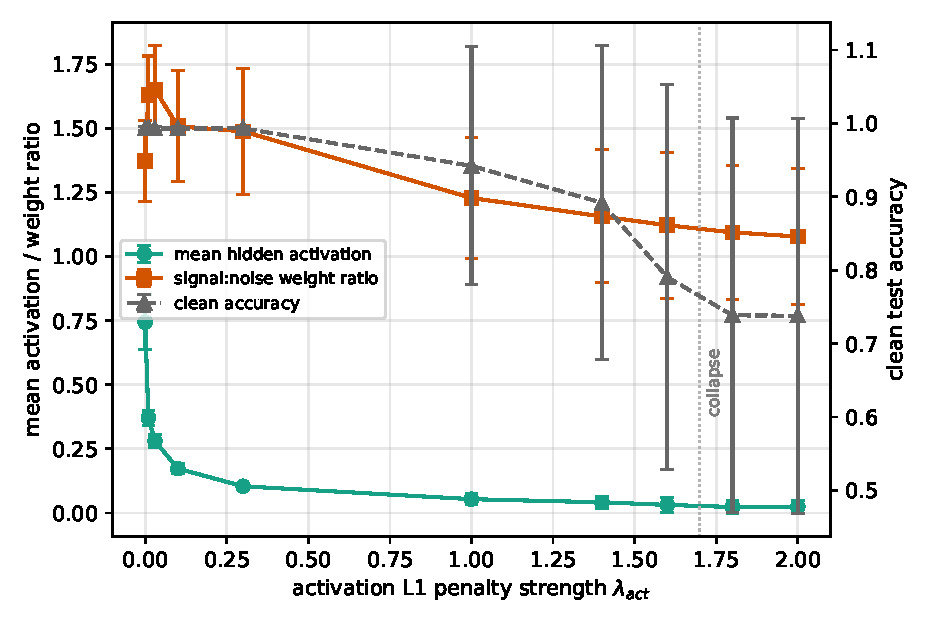
\includegraphics[width=0.62\textwidth]{fig_actsparse_sweep.pdf}
\caption{Mean hidden activation and signal:noise weight ratio (left axis)
vs.\ activation-$L_1$ strength, with clean accuracy (right axis, dashed);
error bars are $\pm 1$ std over 10 seeds. Activation falls smoothly to
zero on average, but the weight ratio stays roughly flat; the widening
accuracy error bars from $\lambda_{\mathrm{act}}\approx1.0$ onward reflect
an increasing fraction of seeds collapsing outright (1/10 at $1.0$ up to
5/10 by $1.8$), not a gradual per-seed decline.}
\label{fig:actsweep}
\end{figure}

We select $\lambda_{\mathrm{act}}=1.4$, a value at which most but not all
seeds remain functional, and compare its attack success rate against Model
A directly (Figure~\ref{fig:actsparsecurves}) rather than relying on the
weight-norm proxy alone. At this $\lambda_{\mathrm{act}}$ (trained here in
the same run as Models A, A-sparse, B, and C, so its specific
initializations differ from the standalone sweep above, which is why the
collapse count differs slightly: 1 of 10 seeds collapsed here against 2 of
10 in the standalone sweep, both being independent samples of the same
seed-dependent phenomenon), a collapsed network has an exactly-zero
gradient everywhere, so FGSM's $\mathrm{sign}(\nabla_x)$ term is
identically zero and its attack success rate is trivially $0.000$ by
construction, a degenerate artifact rather than a meaningful robustness
measurement. We therefore report the attack-success comparison over the 9
non-collapsed seeds only (clean accuracy over those 9: $0.993\pm0.003$);
the full 10-seed mean, diluted by the one degenerate zero-success
collapsed run, would understate the effect described below. Over the 9
functional seeds, \texttt{Aa: non-robust only} ($0.29\pm0.05$ at
$\epsilon=0.3$) is if anything \emph{higher} than \texttt{A: non-robust
only} ($0.23\pm0.02$) --- consistent with the weight norms, where Model
A-actsparse's signal:noise ratio ($\approx 1.0$--$1.3$ across functional
seeds) is actually \emph{lower} than Model A's plain-$L_2$ ratio ($2.41$):
activation sparsity nudged weight allocation slightly more evenly across
all six dimensions, the opposite of what would help. \texttt{Aa: all
dims} ($0.51\pm0.10$) does come out below \texttt{A: all dims}
($0.67\pm0.03$), which is not fully explained by the per-channel breakdown
alone --- we report this rather than force it into a tidier story than
the data supports, and note that the wide standard deviation here
reflects real seed-to-seed variation among the functional networks
themselves (one seed, in particular, put more first-layer weight on two
individual noise dimensions than on the signal dimension, well outside
the range of the other functional seeds), on top of the sharper
collapsed/functional split already discussed. The clear conclusion is the
negative one, scoped to what we actually tested: a mean-activation $L_1$
penalty on a single-hidden-layer ReLU MLP, at any strength that leaves the
network functional, does not reproduce the feature-selection effect that
first-layer weight sparsity produced here, and is additionally less
predictable across random seeds than weight-$L_1$ ever was. We tested one
activation-sparsity mechanism among several standard alternatives (e.g.\
normalized activation penalties, Hoyer-style sparsity, $k$-winners, or
lifetime/sparse-autoencoder-style objectives); we do not claim this
generalizes to activation sparsity as a class, only to the specific
penalty studied here.

\begin{figure}[h]
\centering
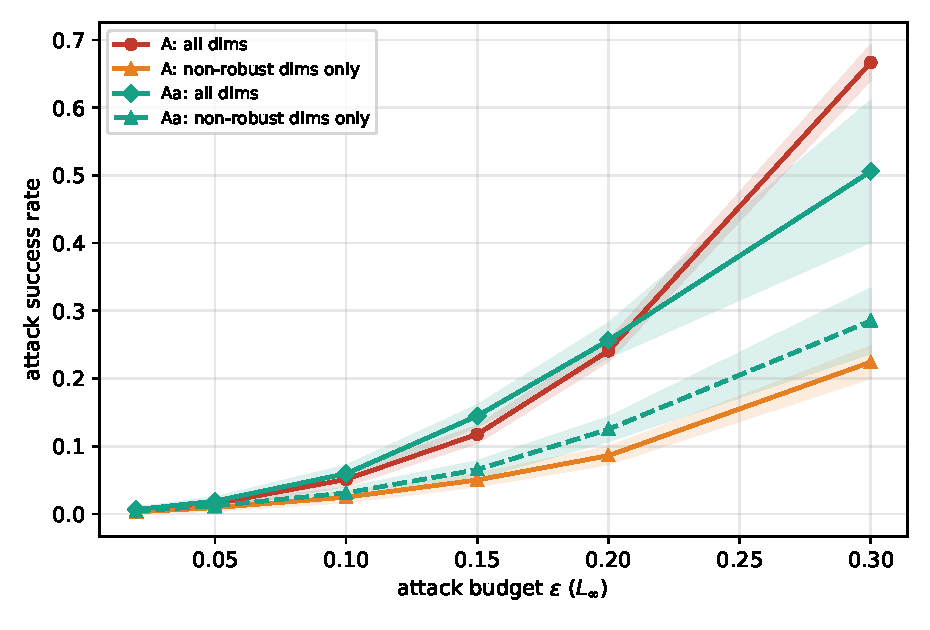
\includegraphics[width=0.72\textwidth]{fig_actsparse_curves.pdf}
\caption{Attack success rate vs.\ budget, Model A vs.\ Model A-actsparse
($\lambda_{\mathrm{act}}=1.4$), overall and restricted to the non-robust
dimensions; mean $\pm 1$ std over the 9 of 10 seeds whose Model
A-actsparse did not collapse (Section~\ref{sec:actsparsity}). The
activation-sparse model's non-robust-only curve sits at or above Model
A's, not below it.}
\label{fig:actsparsecurves}
\end{figure}

\section{An Image-Domain Extension: Circle vs.\ Square}
\label{sec:image}

Everything above hands the network its features as separate scalar input
coordinates -- the network never has to \emph{discover} that dimension $0$
is special. Real images offer no such convenience: whatever plays the role
of a robust or non-robust feature is encoded jointly across many pixels,
and a convolutional network has to extract it. We built a minimal image
analog to test whether the same phenomenon survives that change, and it
surfaced a genuine disanalogy between the two settings that is worth
explaining carefully rather than glossing over.

\subsection{Stimulus and model}

Each $28{\times}28$ grayscale image contains a filled circle (class $0$) or
filled square (class $1$), roughly centered with $\pm 2$ pixel position
jitter, drawn at a fixed bright intensity on a gray background. The
background gray level is generated exactly as the noise dimensions were in
Section~\ref{sec:task}: it shifts with the class but overlaps substantially
across classes, so it is correlated with, but does not determine, the
label. Independent pixel noise is added to the whole image. Shape is the
robust feature (it determines the label by construction); background
level is the non-robust feature (merely correlated). We train a small CNN
(two $3{\times}3$ conv layers with max-pooling, a linear head) with the
same cross-entropy setup as before. Figure~\ref{fig:cleansamples} builds
up the noise sources one at a time from a clean prototype, and
Figure~\ref{fig:stimulusexamples} shows example stimuli as actually used.

\begin{figure}[h]
\centering
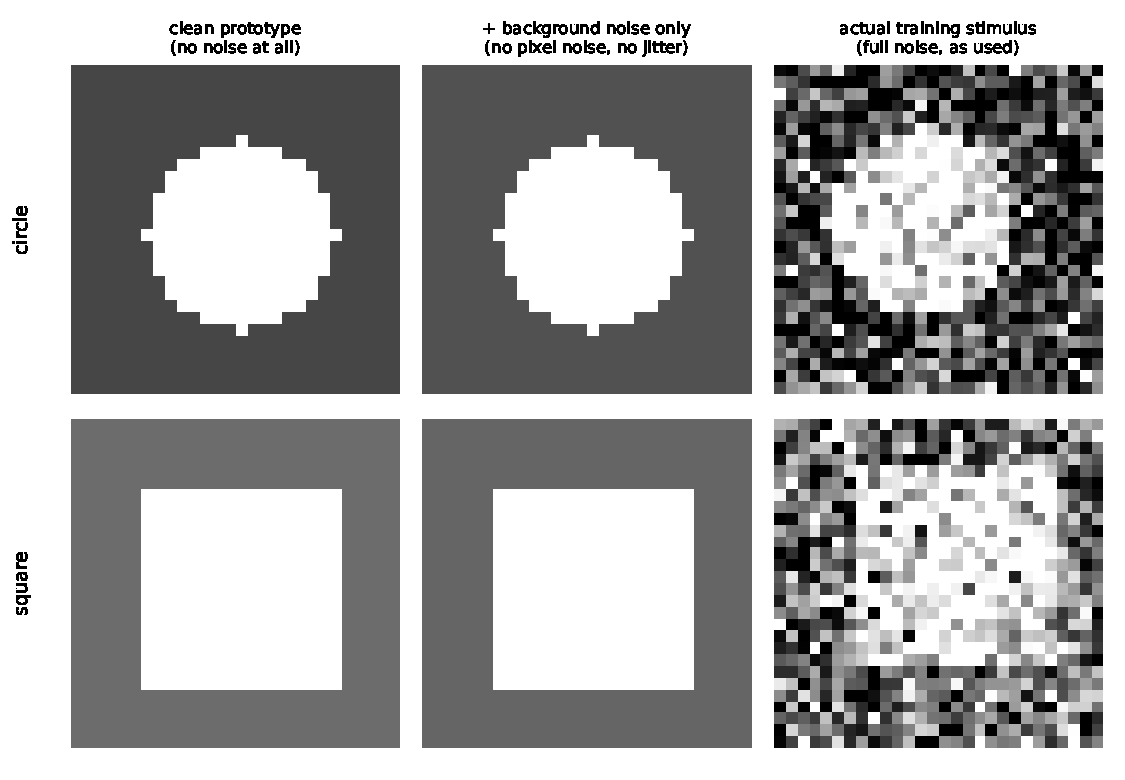
\includegraphics[width=0.78\textwidth]{fig_clean_samples.pdf}
\caption{Left: a noise-free prototype for each class, i.e.\ the shape at a
fixed position on the exact class-conditional mean background level with
no pixel noise -- at this level the background shade difference between
the two classes (the non-robust cue) is visible to the eye. Middle: adding
one sample of background gray-level noise alone (no pixel noise, no
position jitter) barely changes the image. Right: an actual training
stimulus, with pixel noise, position jitter, and background noise all
present as used everywhere else in this section -- the shape is difficult
to make out by eye at all, yet Model A classifies images like this at
$99.6\%\pm0.5$ clean accuracy (Section~\ref{sec:image}), since convolution
spatially averages out the independent per-pixel noise in a way visual
inspection does not.}
\label{fig:cleansamples}
\end{figure}

\begin{figure}[h]
\centering
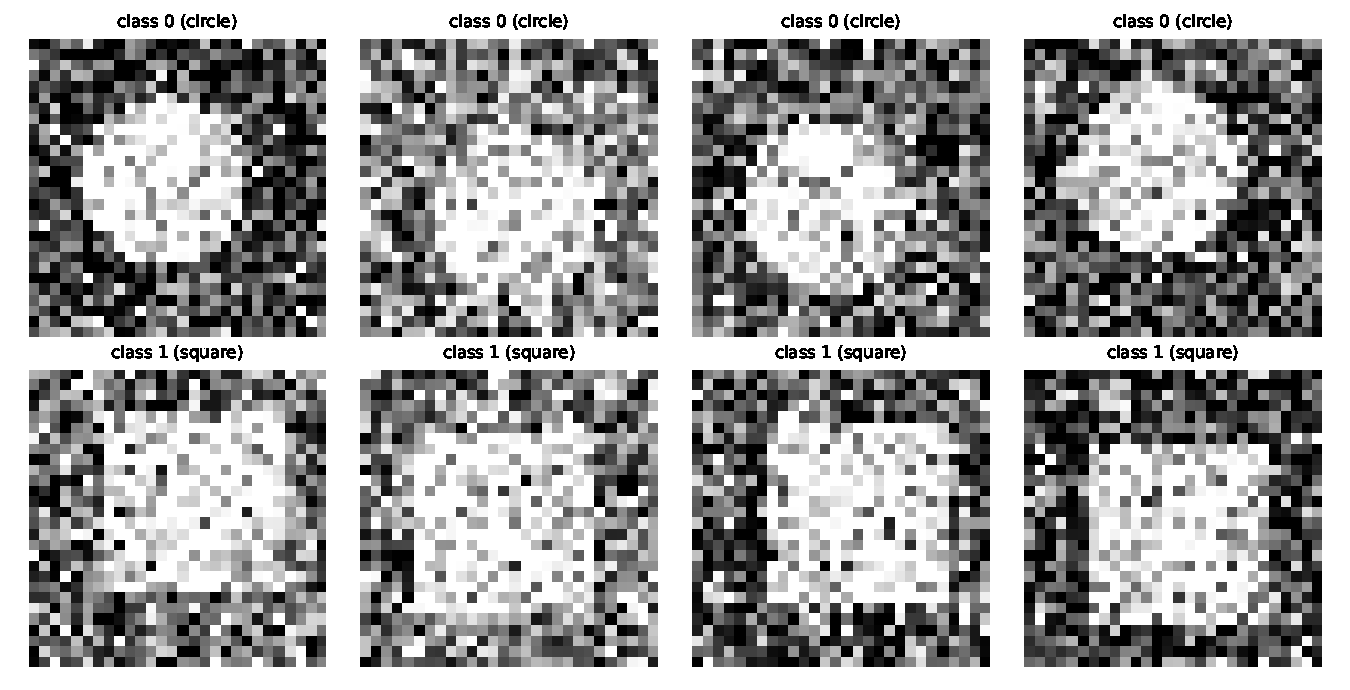
\includegraphics[width=0.85\textwidth]{fig_stimulus_examples.pdf}
\caption{Example stimuli, drawn with the full noise model (as in the
rightmost column of Figure~\ref{fig:cleansamples}). Background gray level
varies within and across classes; it is correlated with class but not
determined by it.}
\label{fig:stimulusexamples}
\end{figure}

\subsection{A domain difference in how the effect appears}

We first calibrated the two cues' individual predictive power the same way
as Table~\ref{tab:sanity}, again averaged over 10 seeds: a model trained on
images with the background forced to a constant value reaches
$99.9\%\pm0.1$ accuracy from shape alone; a model trained on images with
no shape drawn at all reaches $73.8\%\pm1.9$ from background level alone.
Notice that shape-alone accuracy here is far closer to deterministic than
the $95.2\%$ we deliberately engineered for the signal dimension in
Section~\ref{sec:task} --- pixel noise that meaningfully degrades a scalar
feature barely dents a CNN's shape recognition, since convolution
spatially averages out independent pixel noise. By the logic of
Section~\ref{sec:pilot}, this should have suppressed background-cue usage
entirely.

It did not: Model A, trained with both cues present, reaches
$99.6\%\pm0.5$ clean accuracy and is still substantially attackable
through the background cue alone (Table~\ref{tab:image}, discussed
below), consistently across all 10 seeds. Unlike the vector task, a CNN
appears willing to pick up a cheap, globally available correlated signal
even when the dominant cue is nearly deterministic, rather than needing
the dominant cue's imperfection as a precondition. We do not have a full
mechanistic account of why here (finite training, different
capacity/gradient dynamics than the vector MLP, and the low cost of
representing a spatially-uniform cue via pooling are all plausible
contributors) and flag it as an open difference rather than a settled one.

\subsection{Spatial masking, and why "shape region" is not "robust dimension only"}

The vector task could restrict an attack to a single named input
dimension. An image has no such natural seam: the shape's pixels are not
set aside in a separate channel. We approximate the split with two fixed
masks: a central box guaranteed to contain the shape under its position
jitter ("shape region"), and the guaranteed-pure-background border outside
it ("background region").

\begin{table}[h]
\centering
\caption{Model A (image domain) attack success rate by spatial restriction:
mean $\pm$ std over 10 seeds. Clean accuracy $0.996\pm0.005$.}
\label{tab:image}
\begin{tabular}{lccc}
\toprule
$\epsilon$ & all pixels & shape region & background region \\
\midrule
0.05 & 0.325$\pm$0.072 & 0.111$\pm$0.080 & 0.025$\pm$0.033 \\
0.10 & 0.942$\pm$0.037 & 0.587$\pm$0.055 & 0.104$\pm$0.076 \\
0.15 & 0.999$\pm$0.002 & 0.941$\pm$0.032 & 0.266$\pm$0.085 \\
0.20 & 1.000$\pm$0.000 & 0.996$\pm$0.005 & 0.464$\pm$0.073 \\
0.30 & 1.000$\pm$0.000 & 1.000$\pm$0.001 & 0.668$\pm$0.082 \\
0.40 & 1.000$\pm$0.000 & 0.996$\pm$0.013 & 0.711$\pm$0.084 \\
\bottomrule
\end{tabular}
\end{table}

Restricting an attack to the background region alone -- provably never
touching a shape pixel -- still flips on average $46$--$71\%$ of
predictions across $\epsilon=0.2$--$0.4$ (with a standard deviation of
$7$--$8$ points at each budget, reflecting real seed-to-seed variation in
how much the background cue gets used), purely through the correlated,
non-decisive cue. That is the phenomenon from the vector task surviving
intact.

But the "shape region" column is not the image analog of \texttt{A: robust
only}, and reads that way only if the disanalogy is missed. In the vector
task, restricting an attack to the signal dimension still only let the
attacker move one bounded scalar by at most $\epsilon$ -- it could never
let the attacker rewrite what value the underlying generative process had
assigned; a small nudge to $x_0$ is still recognizably close to the true
$x_0$. In the image task, the "shape region" mask covers the same pixels
that constitute the shape's boundary. Perturbing them at a large enough
budget does not nudge a correlate of the true shape -- it can directly
redraw the boundary into something that looks like the other class,
because the boundary pixels \emph{are} the ground truth, not a measurement
of it. Figure~\ref{fig:imageattack} makes this visible directly: the
shape-region attack at $\epsilon=0.2$ visibly distorts the drawn shape,
while the background-region attack changes only the surrounding gray level
and leaves the shape itself untouched.

\begin{figure}[h]
\centering
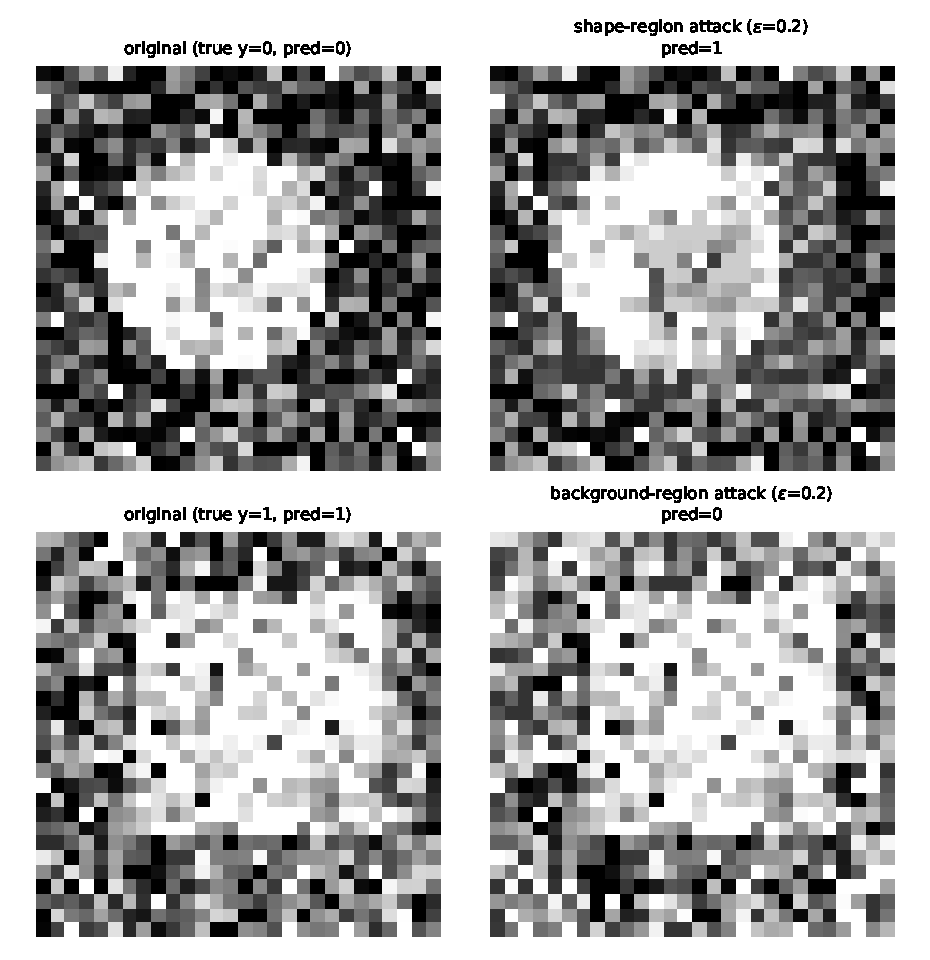
\includegraphics[width=0.62\textwidth]{fig_image_attack_example.pdf}
\caption{One successful attack of each kind on Model A at $\epsilon=0.2$.
Top: restricting the attack to the shape region visibly distorts the shape
itself. Bottom: restricting it to the background region changes only the
surrounding gray level, leaving the shape untouched, and still flips the
prediction.}
\label{fig:imageattack}
\end{figure}

This is a genuine, general point about convolutional/spatial domains, not
a defect specific to this stimulus set: whenever a "robust" feature is
encoded jointly across many pixels rather than isolated in its own input
channel, there is no way to restrict an attack to "that feature's channel
only" without also handing the attacker the power to directly rewrite the
feature itself. The scalar-input formalization used in
Sections~\ref{sec:task}--\ref{sec:actsparsity} (and in the theoretical
constructions of Ilyas et al.\ \cite{ilyas2019} and Tsipras et al.\
\cite{tsipras2018} that it follows) keeps "the channel carrying the robust
feature" and "the mechanism that defines the ground truth" separate by
assumption; raw pixel input does not, and the two collapse into the same
set of pixels whenever the feature is spatially localized. It is also a
reasonable account of why adversarial robustness research bounds
perturbations to a small $L_p$ ball at all: an attacker with a large enough,
unrestricted budget over an object's own pixels is not finding a subtle
non-robust correlate any more, they are simply drawing a different object.
The background-region result is the one that actually matches the intended
sense of "adversarial" -- exploiting an incidental correlate, at a budget
too small to redraw anything -- and it is also the one that survives
faithfully from the vector task to the image domain.

\section{Discussion}

The accuracy/robustness gap between Model A and Model B ($99.2\%\pm0.3$
vs.\ $95.4\%\pm0.7$ clean accuracy, paired with a large gap in attack
success) is a
concrete, fully-attributable instance of the tradeoff Tsipras et al.\
\cite{tsipras2018} describe at a larger scale: a classifier that uses every
feature correlated with the label, including brittle ones, will tend to be
somewhat more accurate and substantially less robust than one restricted to
reliable features. Here we can name exactly which features are responsible
for the difference and exactly how much accuracy they were worth, because
the task was constructed to allow it.

Two points in Sections~\ref{sec:pilot}--\ref{sec:pitfall} are worth
restating as general cautions for similar experiments. The robust/non-robust
mechanism is not automatic: it requires that the reliable feature be
imperfect enough, and the optimizer regularized enough, that the model has
a genuine incentive to also use weaker correlated features --- a perfectly
reliable feature with an unregularized optimizer gives no such incentive,
and the noise dimensions end up dormant and safe by default, which could be
mistaken for a more general finding than it is. Separately, an attack
budget should always be interpreted relative to the feature's own dynamic
range; a budget that spans a large fraction of that range will look like a
robustness failure for reasons having nothing to do with which features are
robust.

\section{Future Work}

The motivating question from the introduction --- whether measured
representational equivariance to a physical transformation predicts natural
adversarial transfer under that same transformation --- is not addressed
here and remains the intended next step. This synthetic task could be
extended toward it directly: define one or more of the "noise" dimensions
as a deterministic but non-identity function of a transform parameter
(e.g.\ a rotation angle), train the same robust/non-robust structure, and
ask whether an attack crafted at one transform value and analytically
transformed to another remains adversarial in proportion to how
equivariant the model's use of that dimension turns out to be. This would
let us test the chain-rule argument sketched in the introduction under full
control, before attempting the same measurement on real self-supervised
vision backbones and real geometric transformations.

\section{Conclusion}

A minimal, fully controlled synthetic task reproduces the robust/non-robust
feature mechanism proposed by Ilyas et al.\ on the smallest scale we could
construct: a model trained on both a reliable and several unreliable
correlated features is measurably more vulnerable through the unreliable
ones, and removing them yields a real, quantifiable robustness gain at a
small accuracy cost. We further showed that this robustness gain does not
require deciding in advance which features are the reliable ones: a
sufficiently strong $L_1$ penalty on the first-layer weights lets the
optimizer discover essentially the same solution on its own, recovering
most of the benefit of explicit removal at broadly similar accuracy,
though with its own version of the same single-point-of-failure tradeoff
observed in the architected case. We also compared this trained model
directly against the exact Bayes-optimal classifier for the same known
generative process (Section~\ref{sec:bayes}): the two are statistically
indistinguishable on clean accuracy, and a model-agnostic permutation-
importance measure shows the trained model relies on the jointly
informative but individually-weak dimensions \emph{less} than a
statistically optimal classifier would, not more --- the vulnerability we
measure throughout this paper is real, but it is not evidence of
over-reliance on those dimensions relative to what the task actually
supports. The weight-sparsity effect is specific to penalizing weights,
not sparsity in general: the one activation-sparsity penalty we tried
(mean-ReLU $L_1$) does not reproduce it at any strength that leaves the
network functional, and instead fails via a dying-ReLU collapse whose
onset is itself seed-dependent rather than a fixed threshold, rather than
trading accuracy for robustness gracefully; we would not extend this
conclusion to activation-sparsity mechanisms we did not test. Extending
the setup to an
image domain (Section~\ref{sec:image}) reproduced the core phenomenon
through a genuinely different mechanism than the vector task did, and
surfaced a real disanalogy worth carrying into any future extension of
this style of experiment: a spatially-distributed robust feature has no
input channel that can be attacked in isolation without also handing the
attacker the power to rewrite the feature itself. Getting a clean version
of these results required several corrections uncovered only by running
the experiments (an imperfect signal feature and, we initially thought,
weight regularization, plus sweeping penalty strength against the correct
baseline rather than guessing a single value) and two interpretive
corrections (excluding an attack budget too large to be meaningful, and
retracting the weight-regularization attribution once the Appendix's
phase diagram isolated it from the signal-reliability change we had
confounded it with).

The appendix subjects the main text's choices to broader checks rather
than leaving them as caveats. A 20-step PGD attack with random restarts
reproduces the vector task's FGSM results exactly (Appendix~\ref{app:pgd})
and the image task's closely, confirming FGSM was not silently
understating either domain's vulnerability. A systematic sweep over
signal reliability, spurious-feature strength, and regularization
strength (Appendix~\ref{app:phase}) shows the effect has a real onset
(vanishing once the signal is reliable enough) and can even invert in a
regime we did not otherwise explore, and overturns our original
weight-decay attribution as just discussed. Group Lasso and elastic net
reproduce $L_1$'s feature-selection benefit about as well as $L_1$ does,
while plain $L_2$ and post-hoc pruning do not
(Appendix~\ref{app:reg}), indicating the effect is about penalizing
input-column magnitude specifically, not about sparsity-inducing
regularization or accuracy cost in general. And an image architecture
with genuine per-cue channel separation, rather than post-hoc spatial
masking of a shared model, measurably reduces the background cue's
exploitability relative to Section~\ref{sec:image}'s single-CNN result,
suggesting Model B's isolation benefit has a real, if less clean, image-domain
counterpart after all (Appendix~\ref{app:twobranch}). All code is
available alongside this note.

\appendix

\section{Appendix: stronger and broader checks}

The main text's central claims (Sections~\ref{sec:main-result}--\ref{sec:image})
rest on a single-step FGSM attack, one point in the generative parameter
space, one regularizer family (weight and activation $L_1$), and a
single-CNN image architecture. This appendix checks each of those choices
directly rather than leaving them as caveats: a multi-step PGD attack
(Appendix~\ref{app:pgd}), a systematic sweep over signal reliability,
spurious-feature strength, and regularization strength
(Appendix~\ref{app:phase}), a comparison against $L_2$, group Lasso,
elastic net, and post-hoc pruning (Appendix~\ref{app:reg}), and an
image-domain architecture with a genuine per-cue channel separation
(Appendix~\ref{app:twobranch}). None of these change the main text's
qualitative conclusions; where they add something new, that is noted
explicitly.

\subsection{PGD vs.\ FGSM}
\label{app:pgd}

We re-attack every model in the vector task (Models A, B, C) with 20-step
$L_\infty$ PGD (step size $\epsilon/4$, 4 random restarts, code in
\texttt{attacks.py} and \texttt{appendix\_pgd.py}), at the same epsilons
and averaged over the same 10 seeds as Table~\ref{tab:main}. The result is
a stronger validation than we expected: PGD-20 produces \emph{exactly} the
same attack success rate as single-step FGSM, at every $\epsilon$, for
every model and restriction, to at least 3 decimal places. We verified
this is not a bug in the PGD implementation by comparing the actual
perturbed points, not just the success rate: for a representative model,
FGSM's and PGD's final adversarial points are identical to floating-point
precision (max per-coordinate difference $0.0$), and a 1-step PGD run
(step size $\epsilon/4$, a quarter of FGSM's step) gives a much lower
success rate as expected, ruling out a silently-inert attack loop.

The explanation is that PGD's advantage over FGSM comes from being able to
change direction partway through the trajectory when the loss surface
curves inside the perturbation ball; here, for this architecture (a single
$8$-unit ReLU hidden layer) and this low-dimensional ($6$-input) task, the
sign of the loss gradient with respect to the perturbed dimensions
apparently does not change between the clean point and the $L_\infty$-ball
boundary FGSM jumps to directly, so iterative refinement has nothing to
correct. This is a property of this specific model class and task, not a
general fact about FGSM being sufficient, and we would not extend it to
larger or deeper networks without checking. For the image-domain CNN,
which is higher-dimensional and more nonlinear, PGD and FGSM are closer to
what one would expect: PGD-20 attack success is at or above FGSM's
background-region and shape-region attack success at every budget we
tested (Table~\ref{tab:pgdimage}), by up to a few points, confirming the
main text's FGSM-based image results are not an artifact of attack
weakness there either, though the two attacks are not identical the way
they are in the vector task. (This image-domain check uses a lighter
PGD-10, 2 restarts, 5 seeds, rather than the vector task's PGD-20/4
restarts/10 seeds, since the CNN makes each PGD step markedly more
expensive; it is a validity check, not a headline result, so we did not
match the vector task's budget exactly.)

\begin{table}[h]
\centering
\caption{Image-domain (Model A) attack success, FGSM vs.\ PGD-10 (2
restarts): mean $\pm$ std over 5 seeds.}
\label{tab:pgdimage}
\begin{tabular}{lcccc}
\toprule
$\epsilon$ & FGSM shape region & PGD shape region & FGSM bg.\ region & PGD bg.\ region \\
\midrule
0.05 & $0.075\pm0.037$ & $0.080\pm0.039$ & $0.015\pm0.012$ & $0.015\pm0.013$ \\
0.10 & $0.558\pm0.044$ & $0.615\pm0.050$ & $0.080\pm0.045$ & $0.087\pm0.047$ \\
0.15 & $0.938\pm0.042$ & $0.974\pm0.027$ & $0.254\pm0.099$ & $0.282\pm0.088$ \\
0.20 & $0.997\pm0.004$ & $1.000\pm0.000$ & $0.447\pm0.115$ & $0.517\pm0.099$ \\
0.30 & $1.000\pm0.000$ & $1.000\pm0.000$ & $0.654\pm0.115$ & $0.752\pm0.090$ \\
0.40 & $1.000\pm0.000$ & $1.000\pm0.000$ & $0.694\pm0.127$ & $0.831\pm0.081$ \\
\bottomrule
\end{tabular}
\end{table}

PGD is at or above FGSM at every budget, most visibly on the
background-region attack at large $\epsilon$ ($0.654 \to 0.752$ at
$\epsilon=0.3$; $0.694 \to 0.831$ at $\epsilon=0.4$, roughly $10$--$14$
points), confirming that in the more nonlinear image setting, unlike the
vector task, FGSM does leave some attack strength on the table --- but
the qualitative pattern the main text reports (background-region attacks
weaker than shape-region, both far above chance) is unchanged under the
stronger attack.

\subsection{A phase diagram over signal reliability, spurious-feature
strength, and regularization}
\label{app:phase}

The main text demonstrates the robust/non-robust effect at one point in
generative-parameter space ($\sigma_0=0.3$, $\alpha=0.4$, weight decay
$10^{-2}$). Here we retrain the Model-A analog on a grid of $\sigma_0 \in
\{0.1,0.2,0.3,0.4,0.5\}$ (signal reliability), $\alpha \in
\{0.1,0.2,0.4,0.6\}$ (spurious-feature strength), and weight decay $\in
\{0, 10^{-3}, 10^{-2}, 10^{-1}\}$ (regularization strength), 5 seeds per
cell, $\sigma_{\mathrm{noise}}=0.25$ held fixed as in the main text (code
in \texttt{phase\_diagram.py}). For each cell we measure clean accuracy,
the signal:noise weight-norm ratio, and FGSM attack success at
$\epsilon=0.2$ restricted to the signal dimension or the noise dimensions.

\begin{figure}[h]
\centering
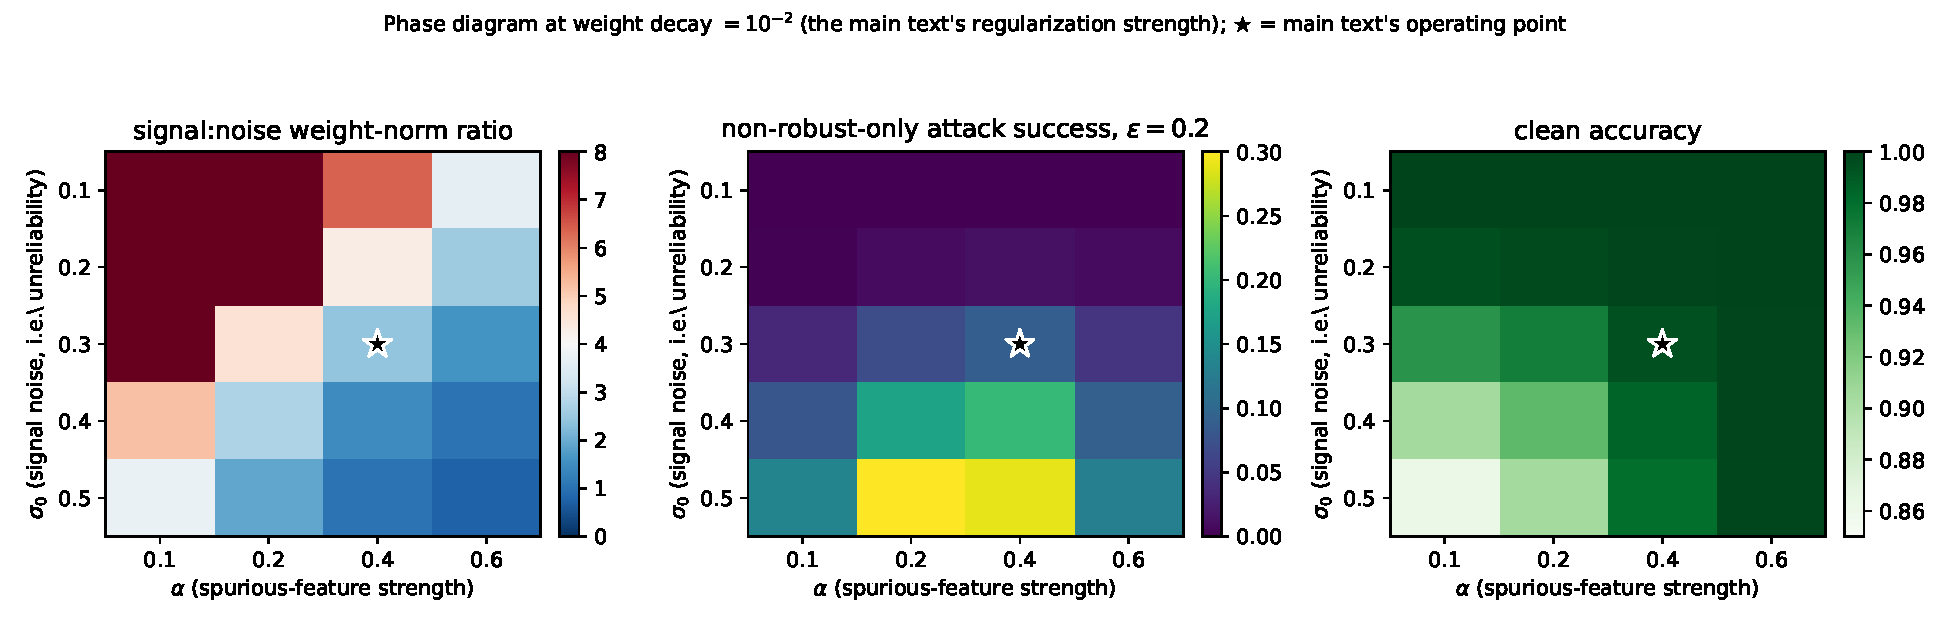
\includegraphics[width=\textwidth]{fig_phase_diagram.pdf}
\caption{Phase diagram at weight decay $=10^{-2}$ (the main text's value),
5 seeds per cell. Left: signal:noise weight-norm ratio. Middle:
non-robust-only attack success at $\epsilon=0.2$ --- this is the
effect's headline signature, and it is far from uniform. Right: clean
accuracy. Star marks the main text's operating point
($\sigma_0=0.3,\alpha=0.4$).}
\label{fig:phasediagram}
\end{figure}

Three things are visible in Figure~\ref{fig:phasediagram} that the main
text's single point does not show. First, the effect has a clear onset:
at $\sigma_0=0.1$ (near-deterministic signal), non-robust-only attack
success is $\approx 0$ everywhere on the $\alpha$/weight-decay grid,
consistent with Section~\ref{sec:pilot}'s pilot finding, and confirming
that finding is not specific to the single $\sigma_0=0.02$ value originally
tested. Second, the effect grows with \emph{both} $\sigma_0$ (a less
reliable signal) and, up to a point, $\alpha$ (a more strongly correlated
spurious feature): non-robust-only attack success reaches $0.405$ at
$\sigma_0=0.5,\alpha=0.2$, far above the main text's $0.089$--$0.131$
region. Third, and unexpectedly, the signal:noise weight ratio can drop
\emph{below} $1$ once the signal is unreliable enough and the spurious
correlation strong enough ($\sigma_0 \ge 0.4$, $\alpha=0.6$: ratio
$0.68$--$1.05$) --- a regime where the model relies more, per dimension,
on an individual noise feature than on the nominally "robust" signal
feature, the qualitative opposite of the main text's setting. We did not
characterize this regime's attack behavior further; it is flagged here as
a boundary case worth a dedicated study, not a claim we substantiate.

The weight-decay sweep produced the more consequential correction,
already discussed in Section~\ref{sec:pilot}: at fixed $\sigma_0$ and
$\alpha$, increasing weight decay from $0$ to $10^{-1}$ \emph{monotonically
decreases} non-robust-only attack success in every row we checked (e.g.\
at $\sigma_0=0.5,\alpha=0.1$: $0.211 \to 0.205 \to 0.136 \to 0.040$ as
weight decay increases), the opposite of the direction our original,
single-point pilot experiment led us to assume. Weight decay is not the
active ingredient that unlocks the effect; an imperfect signal is
sufficient on its own, and weight decay -- like the feature-selection
regularizers of Appendix~\ref{app:reg}, though far more weakly -- pushes
in the direction of \emph{suppressing} reliance on the individually-weaker
noise dimensions, not amplifying it.

\subsection{Regularizer comparison: $L_1$ vs.\ $L_2$, group Lasso, elastic
net, and pruning}
\label{app:reg}

Section~\ref{sec:sparsity}'s first-layer $L_1$ penalty is one specific
choice; here we compare it against $L_2$ (weight decay) at several
strengths, group Lasso ($\sum_i \lVert W^{(1)}_{:,i} \rVert_2$, an $L_1$
norm over per-dimension $L_2$ norms --- the theoretically natural
feature-selection penalty when whole input \emph{columns}, not individual
weights, are the unit of interest), elastic net ($L_1$ fixed at $0.1$
with $L_2$ swept), and post-hoc magnitude pruning of the smallest-norm
input columns with no retraining afterward (code in
\texttt{regularizer\_comparison.py}, 10 seeds per point). Each method is
swept over a strength grid and we report the point closest to Model
A-sparse's operating accuracy ($0.966$, $\lambda_{L_1}=0.4$), so all five
methods are compared at matched accuracy as in Section~\ref{sec:sparsity}.

\begin{table}[h]
\centering
\caption{Matched-accuracy comparison ($\text{target accuracy} \approx
0.966$): mean $\pm$ std over 10 seeds, attack success at $\epsilon=0.3$.}
\label{tab:regcomparison}
\begin{tabular}{lccccc}
\toprule
Method & Strength & Accuracy & Sig.:noise ratio & Robust-only & Non-robust-only \\
\midrule
$L_1$ (Section~\ref{sec:sparsity}) & $0.4$ & $0.966\pm0.006$ & $\approx 20.4$ & $0.182\pm0.015$ & $0.018\pm0.008$ \\
Group Lasso & $0.4$ & $0.970\pm0.005$ & $18.88\pm5.14$ & $0.168\pm0.016$ & $0.027\pm0.008$ \\
Elastic net & $L_2=0.01$ & $0.973\pm0.004$ & $14.28\pm2.44$ & $0.161\pm0.010$ & $0.034\pm0.007$ \\
$L_2$ only & $0.2$ & $0.964\pm0.008$ & $2.72\pm0.03$ & $0.127\pm0.012$ & $0.344\pm0.020$ \\
Pruning (no retrain) & $k=1$ & $0.982\pm0.004$ & $2.96\pm0.10$ & $0.080\pm0.008$ & $0.204\pm0.015$ \\
\bottomrule
\end{tabular}
\end{table}

Two findings survive this broader comparison and one complicates the main
text's story usefully. First, the $L_1$ result is not an accident of
using elementwise $L_1$ specifically: group Lasso and elastic net both
reach a comparable signal:noise ratio ($\approx 14$--$19$, against
$L_1$'s $\approx 20$) and comparably low non-robust-only attack success
($0.027$--$0.034$, against $L_1$'s $0.018$) at matched accuracy, and
group Lasso is if anything the more principled choice for this task,
since its penalty structure matches the actual unit being selected (a
whole input dimension, not an individual weight). Second, plain $L_2$
does not reproduce the effect at any strength: pushed hard enough to
match the sparse methods' accuracy cost ($0.964$ at weight decay $0.2$),
its non-robust-only attack success is $0.344$ --- \emph{higher} than
Model A's own baseline weight decay of $10^{-2}$ ($0.224$, Table
\ref{tab:main}) --- meaning simply increasing $L_2$ strength trades away
accuracy \emph{without} buying any robustness, a strictly worse operating
point than doing nothing; pushed further still ($\ge 0.4$), the model
collapses to chance-level accuracy ($\approx 0.49$) rather than
degrading gracefully, a different failure mode from
Section~\ref{sec:actsparsity}'s dying-ReLU collapse but similarly abrupt.

The complication is post-hoc pruning. Pruning just the single
smallest-norm noise column, with no fine-tuning afterward, already costs
more accuracy relative to its own un-pruned baseline than any training-time
method here, while barely reducing non-robust-only attack success
($0.204$, against the unpruned baseline's $0.224$) --- the remaining four
noise columns are still fully able to carry the correlation the attacker
exploits, and removing one column's worth of capacity has nowhere to
redistribute to without retraining. The next pruning step ($k=2$) costs a
further $4.3$ accuracy points ($0.982 \to 0.939$), a much steeper
accuracy cost per unit of noise-dimension removed than $L_1$ or group
Lasso pay for removing all five smoothly. Post-hoc pruning without
retraining is, at least in this task, a distinctly worse tool than any of
the training-time penalties, and we would not generalize the sparsity
comparisons above to a pruning setup that included fine-tuning, which we
did not test.

\subsection{An image architecture with a genuine per-cue channel
separation}
\label{app:twobranch}

Section~\ref{sec:image}'s disanalogy arises because a single shared CNN
sees the whole image, so restricting an attack to a spatial region is not
the same as restricting it to an input \emph{channel} the way masking a
vector dimension is: the shared model can still combine information from
both regions however it likes. We built a two-branch CNN where that is no
longer true by construction: a shape branch that receives only the
cropped shape-region pixels ($20\times20$, guaranteed to contain the
shape under its position jitter), and a background branch that receives
the full image with that same region zeroed out, each processed by its
own small two-conv-layer tower into a 16-dimensional feature vector, the
two concatenated before a shared linear head (code and full architecture
in \texttt{image\_two\_branch.py}). Because the two branches' weights
never see each other's region at all, restricting a perturbation to one
region now restricts it to one branch's \emph{entire} input, the genuine
image-domain analog of Model A's per-dimension masking --- not merely a
spatial subset of one shared model's input, as in Section~\ref{sec:image}.
We trained this on the same generative image task, 5 seeds (fewer than
the main text's 10, since the two-branch model roughly doubles training
cost).

\begin{table}[h]
\centering
\caption{Two-branch CNN, channel-restricted attack success: mean $\pm$
std over 5 seeds. Clean accuracy $0.997\pm0.002$, comparable to the
single-CNN Model A's $0.996\pm0.005$.}
\label{tab:twobranch}
\begin{tabular}{lcccc}
\toprule
$\epsilon$ & FGSM shape branch & FGSM bg.\ branch & PGD shape branch & PGD bg.\ branch \\
\midrule
0.05 & $0.082\pm0.043$ & $0.007\pm0.004$ & $0.086\pm0.044$ & $0.007\pm0.004$ \\
0.10 & $0.502\pm0.078$ & $0.026\pm0.013$ & $0.572\pm0.076$ & $0.027\pm0.013$ \\
0.15 & $0.901\pm0.051$ & $0.071\pm0.025$ & $0.969\pm0.025$ & $0.079\pm0.031$ \\
0.20 & $0.987\pm0.016$ & $0.142\pm0.069$ & $1.000\pm0.000$ & $0.162\pm0.079$ \\
0.30 & $0.995\pm0.011$ & $0.312\pm0.130$ & $1.000\pm0.000$ & $0.357\pm0.154$ \\
0.40 & $0.968\pm0.071$ & $0.454\pm0.175$ & $1.000\pm0.000$ & $0.523\pm0.197$ \\
\bottomrule
\end{tabular}
\end{table}

Two patterns emerge, one confirming the main text and one adding to it.
The shape-branch attack remains highly effective at every budget
($0.90$--$1.00$ from $\epsilon=0.15$ up), consistent with
Section~\ref{sec:image}'s point that shape pixels are the ground truth,
not a measurement of it --- architectural isolation of the shape channel
does not change this, because the problem was never that the shape
channel was entangled with the background channel, it is that perturbing
shape pixels at a large enough budget redraws the shape regardless of
what else the model sees. The background-branch attack, in contrast, is
\emph{substantially weaker here than the single-CNN's background-region
attack at every budget} ($0.312$ vs.\ $0.668$ at $\epsilon=0.3$; $0.454$
vs.\ $0.711$ at $\epsilon=0.4$, both from Table~\ref{tab:image}) despite
comparable clean accuracy. This is the positive result the reviewer's
suggestion was aiming at: genuine architectural channel separation, not
just post-hoc spatial masking of a shared model, measurably reduces how
exploitable the non-robust (background) cue is, in the same direction
as Model B's isolation benefit over Model A in the vector task.

We would not over-claim this as a clean, controlled ablation, though: the
two-branch model has roughly twice the convolutional parameters of the
single-CNN Model A (two independent towers rather than one), so we cannot
rule out that some of the reduction is a capacity or bottleneck effect
(each branch's 16-dimensional feature vector is a narrower channel into
the shared head than the single CNN's direct route to its output layer)
rather than purely the channel separation itself, and 5 seeds is fewer
than we would want for a confident effect size. We report the direction
and magnitude honestly rather than treating this as a settled result;
disentangling capacity from separation as the driver is a natural next
step we did not take here.

\begin{thebibliography}{9}

\bibitem{lu2019dying}
L.~Lu, Y.~Shin, Y.~Su, G.~E.~Karniadakis.
\emph{Dying ReLU and Initialization: Theory and Numerical Examples}.
Communications in Computational Physics, 2020 (arXiv:1903.06733).

\bibitem{tibshirani1996}
R.~Tibshirani.
\emph{Regression Shrinkage and Selection via the Lasso}.
Journal of the Royal Statistical Society, Series B, 1996.

\bibitem{szegedy2014}
C.~Szegedy, W.~Zaremba, I.~Sutskever, J.~Bruna, D.~Erhan, I.~Goodfellow,
R.~Fergus.
\emph{Intriguing properties of neural networks}.
ICLR, 2014.

\bibitem{goodfellow2015}
I.~Goodfellow, J.~Shlens, C.~Szegedy.
\emph{Explaining and Harnessing Adversarial Examples}.
ICLR, 2015.

\bibitem{madry2018}
A.~Madry, A.~Makelov, L.~Schmidt, D.~Tsipras, A.~Vladu.
\emph{Towards Deep Learning Models Resistant to Adversarial Attacks}.
ICLR, 2018.

\bibitem{ilyas2019}
A.~Ilyas, S.~Santurkar, D.~Tsipras, L.~Engstrom, B.~Tran, A.~Madry.
\emph{Adversarial Examples Are Not Bugs, They Are Features}.
NeurIPS, 2019.

\bibitem{tsipras2018}
D.~Tsipras, S.~Santurkar, L.~Engstrom, A.~Turner, A.~Madry.
\emph{Robustness May Be at Odds with Accuracy}.
ICLR, 2019.

\bibitem{athalye2018}
A.~Athalye, N.~Carlini, D.~Wagner.
\emph{Obfuscated Gradients Give a False Sense of Security: Circumventing
Defenses to Adversarial Examples}.
ICML, 2018.

\end{thebibliography}

\end{document}
